\documentclass[ASNA,twocolumn]{USG} %twocolumn
\usepackage{anyfontsize} %
\usepackage{pgfplots}
\pgfplotsset{compat=1.18} % Assure la compatibilité des graphiques
\usepackage{colortbl}   % For coloring table lines
\usepackage{xcolor}     % For color definitions
\usepackage{tikz}
\usetikzlibrary{shapes.geometric, arrows.meta, positioning, fit, calc}
\usepackage{steinmetz}
\graphicspath{{./images/}}
\usepackage{graphicx}
\usepackage{algorithm}
\usepackage{url}
\usepackage{listings}
\usepackage{booktabs}
\usepackage{multirow}
\usepackage{xstring} 
\usepackage{hyperref}
\usepackage{algpseudocode} % Plus moderne et compatible avec Wiley
%\specialissue{} 
\usepackage{subcaption}
\articletype{ORIGINAL ARTICLE}%
\subarticletype{Knowledge Engineering and Artificial Intelligence} 
\received{00 Month 2026} 
\revised{00 Month 2026}  
\accepted{00 Month 2026} 
\journal{Expert Systems} 
\volume{0}
\copyyear{2026} 
\startpage{1}
\articledoi{} 
\raggedbottom
%\raggedbottom

%%
%\renewcommand\ShowFrameLinethickness{0.15pt}
%\renewcommand*\ShowFrameColor{\color{red}}
% Conforme Wiley Expert Systems
\lstdefinestyle{xcarecode}{
  basicstyle=\fontsize{7.5}{9.5}\selectfont\ttfamily,
  breaklines=true,
  breakatwhitespace=false,
  keepspaces=true,
  columns=flexible,
}
% ====================================================================
% ====================================================================
\begin{document}

\title{AILS: An Adaptive  Intelligent Tutoring System with
       Real-Time Cognitive Load Detection, Hybrid Recommendation,
       and SHAP-Based Explainability --- Extended Validation with
       Real-World Experimental Protocol}

\author[1]{Sabrine OUERIECH}
\author[1,2]{Nacim YANES}
\author[1]{Mabrouka CHOUCHANE}

\authormark{OUERIECH \textsc{et al.}}
\titlemark{AILS: ADAPTIVE IMMERSIVE INTELLIGENT TUTORING SYSTEM}

\address[1]{%
  \orgdiv{ISGGB,}
  \orgname{University of Gabès,}
  \orgaddress{\state{Gabès 6002,} \country{Tunisia}}}

\address[2]{%
  \orgdiv{RIADI Lab.\ (LR99ES26), ENSI,}
  \orgname{Manouba University,}
  \orgaddress{\state{Manouba 2010,} \country{Tunisia}}}

\corres{Nacim Yanes (\email{nacim.yanes@ensi-uma.tn})}

\keywords{intelligent tutoring systems | adaptive learning |
          virtual reality | cognitive load | collaborative filtering |
          large language models | explainable AI | SHAP |
          experimental validation}

\keywords{intelligent tutoring systems | adaptive learning |
          virtual reality | cognitive load | collaborative filtering |
          large language models | explainable AI | SHAP |
          experimental validation}

%% ── FIX 1: abstract threshold updated 0.65 → 0.60 ──────────────────
\abstract[ABSTRACT]{%
Intelligent Tutoring Systems (ITS) have demonstrated strong potential
for personalized learning; however, two key limitations persist:
(i)~the absence of real-time cognitive load (CL) monitoring within a
closed adaptive loop, and (ii)~the lack of transparency in
recommendation decisions.
This paper presents AILS (Adaptive Immersive Learning System), a
unified ITS architecture designed for immersive Virtual Reality (VR)
environments that addresses both challenges through a dual-loop
design. The intra-module loop dynamically classifies learner error
types and estimates cognitive load using multimodal behavioral signals.
Based on these inputs, a large language model (LLM) generates
personalized exercises via few-shot prompting. The inter-module loop
leverages collaborative filtering to recommend subsequent learning
modules according to behavioral similarity across learners.
SHAP-based explainable AI is integrated to quantify the contribution
of each behavioral feature to adaptation decisions.
The architecture is first validated through a controlled end-to-end
synthetic simulation over a ten-module Baccalaureate Informatics
curriculum ($N{=}30$ synthetic profiles), achieving $+217\%$ learning
gain over the static baseline with a $46\%$ cognitive load reduction.
This extended version reports a real-world evaluation conducted with
$N{=}34$ Tunisian Baccalaureate students under real classroom
conditions, employing four psychometrically validated
instruments: a Learner Profile Questionnaire, a Post-Exercise
Cognitive Load Questionnaire (adapted from NASA-TLX and Paas scales),
an Expert Evaluation Questionnaire ($\kappa \geq 0.70$), and an
Explanation Satisfaction Questionnaire. Content validity was confirmed
by a three-expert panel (CVI\,=\,1.0), and internal consistency
established by pilot study ($\alpha > 0.70$ on all scales).}

\abbr{AILS, Adaptive Immersive Learning System; BKT, Bayesian
Knowledge Tracing; CF, Collaborative Filtering; CL, Cognitive Load;
CLT, Cognitive Load Theory; CVI, Content Validity Index; ESS,
Explanation Satisfaction Scale; ITS, Intelligent Tutoring System;
LLM, Large Language Model; NASA-TLX, NASA Task Load Index; SHAP,
SHapley Additive exPlanations; VR, Virtual Reality; XAI, Explainable
Artificial Intelligence.}

\maketitle
\section{Introduction}
\label{sec:intro}
% ====================================================================

Intelligent Tutoring Systems (ITS) represent one of the most
active frontiers in educational technology, aiming to replicate
the adaptive quality of one-to-one human tutoring through
automated learner modelling and content personalisation
\cite{Corbett1995}.
Over three decades of research, ITS architectures have evolved
from simple rule-based systems to probabilistic models ---
most notably Bayesian Knowledge Tracing (BKT)
\cite{Corbett1995} --- and more recently to deep-learning
approaches capable of processing rich interaction histories
\cite{Piech2015,Ghosh2020}.
The deployment of ITS in immersive Virtual Reality (VR)
environments further extends this potential: the rich sensory
context fosters presence and agency \cite{Makransky2021},
enabling learners to interact with abstract concepts in
three-dimensional spaces unavailable to conventional
instructional media \cite{Marougkas2024}.
Yet across this evolution, two structural limitations have
proved persistently difficult to resolve.

% ── 1.1 ──────────────────────────────────────────────────────────────
\subsection{Problem and Dual Bottleneck}
\label{sec:intro_problem}

The first limitation is the \emph{cognitive blindness} of
most adaptive engines: they respond to observable performance
indicators but remain agnostic to the learner's internal
cognitive state.
Cognitive Load Theory (CLT) \cite{Sweller1988} has long
established that the efficiency of learning depends not only
on performance outcomes but on the cognitive resources consumed
to achieve them.
Two decades of empirical evidence confirm that instruments
derived from NASA-TLX \cite{Hart1988} and Paas mental effort
scales \cite{Paas1992} reliably capture this workload, yet
these measurements have rarely been operationalised within
real-time closed adaptive loops.
Recent multimodal estimation approaches using oculometrics
\cite{Suzuki2024,Xue2024} demonstrate the technical
feasibility of continuous CL monitoring, but none integrates
these signals into a recommendation engine that actively adjusts
exercise selection in response to detected cognitive overload.
The second limitation is the \emph{opacity} of recommendation
decisions.
Modern adaptive systems function as black boxes, selecting
exercises or adjusting difficulty without providing the learner
or the instructor with any justification.
Post-hoc XAI techniques such as SHAP \cite{Lundberg2017} and
LIME \cite{Ribeiro2016} produce numerical feature importance
arrays that, while statistically rigorous, lack the semantic
grounding required for pedagogical decision-making.
Govea et al.\ \cite{Govea2024} demonstrated that
XAI-augmented recommenders significantly improve both
recommendation precision and user trust in educational
contexts, yet their integration into ITS architectures ---
particularly immersive ones --- remains largely absent from
the literature \cite{Khosravi2022}.

To address this dual algorithmic and pedagogical gap, this
paper presents \textbf{AILS} (Adaptive Immersive Learning
System), a unified ITS architecture built upon two
synergistic adaptive loops.

The \emph{intra-module loop} addresses algorithmic
responsiveness: it dynamically classifies learner error types,
estimates cognitive load from multimodal behavioral signals,
and generates personalised exercises via a two-layer
structured prompt to the Mistral large language model (LLM)
\cite{Said2024}, enriched by Retrieval-Augmented Generation
(RAG) from a validated Baccalaureate exercise corpus.
Rather than applying a static difficulty adjustment, the
intra-module engine scales exercise complexity and hint
provision in real time as a function of the detected CL state,
following a dynamic weight schedule that prioritises CL relief
over content optimality when cognitive overload is detected.

The \emph{inter-module loop} addresses strategic progression:
it recommends the next learning module based on behaviorally
enriched collaborative filtering (CF), drawing on peer
similarity across a profile space that encodes not only
performance scores but cognitive load history, error
distribution, and mastery progression.
Upon each inter-module transition, a dual-level XAI layer
generates both a learner-facing natural-language explanation
--- derived from SHAP-based attribution values computed via
a \texttt{KernelExplainer} applied to a
\texttt{GradientBoostingRegressor} trained on interaction
history --- and a teacher-facing structured log, implementing
a two-audience explainability strategy that preserves Human-in-the-Loop
(HITL) oversight while maintaining pedagogical transparency
for the learner.

% ── 1.2 ──────────────────────────────────────────────────────────────
\subsection{Research Questions}
\label{sec:intro_rq}

The empirical design of this study is structured around two
primary research questions:

\begin{enumerate}[(1)]
  \item \textbf{RQ1.}
        Does the AILS dual-loop architecture --- combining
        real-time CL-driven exercise adaptation with
        behaviorally enriched CF-based module recommendation
        --- produce statistically significant learning gain
        and cognitive load reduction compared to non-adaptive
        and partially adaptive baselines?

  \item \textbf{RQ2.}
        Does the SHAP-based two-audience explainability
        strategy generate pedagogically trustworthy,
        structurally adherent, and learner-perceived useful
        explanations, as verified by expert evaluation and
        Explanation Satisfaction Scale measurement?
\end{enumerate}

% ── 1.3 ──────────────────────────────────────────────────────────────
\subsection{Core Contributions}
\label{sec:intro_contributions}

This research makes the following original contributions to
the literature at the intersection of adaptive learning,
explainable AI, and intelligent tutoring systems:

\begin{enumerate}[1.]

  \item \textbf{Dual-Loop CL-Adaptive Architecture.}
        We propose and empirically validate a dual-loop
        adaptive engine that simultaneously integrates
        real-time cognitive load estimation, LLM-based
        personalised exercise generation, and
        behaviorally enriched collaborative filtering ---
        an architectural combination absent from existing
        ITS literature, as confirmed by the comparative
        analysis of 25 representative systems
        (Table~\ref{tab:comparison}).

  \item \textbf{Dynamic CL-Driven Weight Schedule.}
        We design and validate a topology-aware fusion weight
        schedule (Eq.~\eqref{eq:fusion_weights}) that
        autonomously scales the relative priority of
        CL-relief versus content-based signals according to
        three runtime states (cold-start, CL-critical,
        steady-state), supported by a sensitivity analysis
        across eight weight configurations
        (Table~\ref{tab:weight_sensitivity}).

  \item \textbf{Two-Audience SHAP Explainability.}
        We engineer a SHAP-based attribution pipeline
        (Eq.~\eqref{eq:shap}) applied to a
        \texttt{GradientBoostingRegressor} trained on
        learner interaction history, producing
        instance-level feature attributions that are
        simultaneously translated into learner-facing
        natural-language messages
        (Table~\ref{tab:shap_mapping}) and
        teacher-facing structured logs --- demonstrating
        through Mann-Whitney evaluation ($p{=}0.013$,
        $d{=}0.71$) that the explanations produce a
        significant increase in perceived trust and utility.

  \item \textbf{Anti-Hallucination LLM Pipeline.}
        We implement a layered JSON sanitisation and
        Verification Engine ($\kappa \geq 0.70$) that
        systematically intercepts three LLM hallucination
        failure modes (format deviation, control-character
        injection, structural incompleteness) before
        pedagogical content checks, achieving an expert
        quality score of $4.22/5$ with inter-rater
        reliability $\kappa{=}0.74$.

  \item \textbf{Real-World Classroom Validation.}
        We present the results of a live pilot study with
        $N{=}34$ Tunisian Baccalaureate Informatics
        students, yielding a statistically significant
        learning gain ($W{=}117.5$, $p{=}0.0005$;
        Cohen's $d{=}0.67$) and confirming the system's
        feasibility under authentic classroom conditions
        without specialised sensor infrastructure.

  \item \textbf{Open Reproducibility.}
        The complete AILS codebase --- including the
        Gradio-based classroom interface, Google Sheets
        real-time ingestion pipeline, dynamic CF engine,
        and SHAP attribution module --- is publicly
        released, enabling full scientific reproducibility
        and future benchmarking against the evaluation
        framework defined in Section~\ref{sec:evaluation}.

\end{enumerate}

% ── 1.4 ──────────────────────────────────────────────────────────────
\subsection{Extension Statement}
\label{sec:intro_extension}

This manuscript represents a substantial extension of the
preliminary architecture presented at the KES~2026
conference \cite{Loussaief2026}.
While the conference proceedings established the
proof-of-concept for the intra-module loop on a single
synthetic drift scenario and demonstrated an operational
LLM generation pipeline, this article introduces four
significant novel contributions.
First, we extend the empirical evaluation to a
real-world deployment with $N{=}34$ live participants,
transitioning the architecture from offline simulation
to authentic classroom validation.
Second, we introduce the inter-module CF loop with
behaviorally enriched peer similarity, which was absent
from the conference version.
Third, we engineer the full two-audience SHAP
explainability strategy with a
\texttt{GradientBoostingRegressor}-based
\texttt{KernelExplainer}, replacing the closed-form
heuristic attribution of the original prototype.
Fourth, we provide a systematic LLM quality audit
through expert evaluation ($N_e{=}3$, $\kappa{=}0.74$)
and Explanation Satisfaction Scale measurement
($n{=}34$, Mann-Whitney $p{=}0.013$).

% ── 1.5 ──────────────────────────────────────────────────────────────
\subsection{Paper Organisation}
\label{sec:intro_organisation}

The remainder of this paper is organised as follows.
Section~\ref{sec:background} critically reviews related
work across four converging domains: ITS and learner
modelling, cognitive load measurement, LLM-based exercise
generation, and explainable AI in adaptive education.
Section~\ref{sec:architecture} details the mathematical
formulation of the dual-loop engine, the dynamic CL
weight schedule, the two-layer LLM prompt architecture,
and the two-audience SHAP explainability strategy.
Section~\ref{sec:evaluation} defines the validation
framework with a priori thresholds across four
evaluation dimensions.
Section~\ref{sec:synthetic_validation} presents the
synthetic simulation results over $N{=}30$ profiles and
ten curriculum modules.
Section~\ref{sec:realworld} presents the real-world
deployment protocol and experimental results
($N{=}34$ students).
Section~\ref{sec:discussion} discusses key design
choices, limitations, and future directions, and
Section~\ref{sec:conclusion} concludes the paper.
% ====================================================================
\section{Related Work}
\label{sec:background}
% ====================================================================

\subsection{ITS and Learner Modeling}

ITS research has progressively enriched learner models from binary
mastery estimates (BKT \cite{Corbett1995}) to probabilistic extensions
incorporating response time and performance trends \cite{Cai2022}.
Deep Knowledge Tracing (DKT) \cite{Piech2015} replaced hand-crafted
knowledge components with recurrent neural networks; subsequent
variants such as SAKT \cite{Pandey2019} and AKT
\cite{Ghosh2020} introduced attention mechanisms to capture
long-range dependencies between exercise interactions.
Despite strong predictive accuracy, these models remain opaque
and provide no actionable pedagogical feedback.

More recently, Abdelrahman et al.\ \cite{Abdelrahman2023}
proposed a contrastive learning extension of knowledge tracing
(CL-KT) that improves skill generalisation across domains but
still lacks any adaptation mechanism beyond score prediction.
Long et al.\ \cite{Long2022} introduced CORE, a
context-aware knowledge tracing model that incorporates
exercise difficulty and learner fatigue into the prediction
objective --- the first KT model to explicitly account for
cognitive state, though without closing the loop into a
recommendation engine.
Hybrid recommendation approaches combining collaborative and
content-based filtering consistently outperform single-strategy
systems \cite{Khanal2020}.
Liu et al.\ \cite{Liu2023} propose a knowledge-graph-enhanced
recommender that enriches learner profiles with prerequisite
relationships between concepts, improving recommendation
relevance in structured curricula --- architecturally close to
AILS's directed acyclic graph of module prerequisites, though
without CL awareness or XAI transparency.
Marougkas et al.\ \cite{Marougkas2024} further show that
personalised immersive VR environments improve engagement and
learning outcomes, yet their adaptation logic remains
score-driven and lacks cognitive state awareness.

\subsection{Cognitive Load Measurement in Digital Learning}

CLT \cite{Sweller1988} partitions cognitive load into intrinsic,
extraneous, and germane components.
The NASA-TLX \cite{Hart1988} is the reference subjective
instrument for workload assessment; single-item effort ratings
further demonstrate high sensitivity in instructional contexts
\cite{Paas1992}.

For real-time objective estimation, oculometric indicators
constitute validated behavioral proxies
\cite{Suzuki2024,Xue2024}.
Shi et al.\ \cite{Shi2023} demonstrate that pupil dilation and
fixation duration measured via low-cost eye trackers correlate
significantly with NASA-TLX scores ($r{=}0.68$) during
programming exercises, directly motivating AILS's use of gaze
direction $\hat{g}$ as a CL proxy channel.
Lim et al.\ \cite{Lim2023} propose a multimodal CL estimator
combining EEG and eye-tracking signals in an online learning
environment, achieving classification accuracy of $82\%$
across four cognitive states --- consistent with the four-state
taxonomy (Confidence, Exploration, Hesitation, Confusion)
adopted in AILS.

In VR contexts, CAMIL \cite{Makransky2021} establishes that
immersive environments amplify extraneous load; Parong and
Mayer \cite{Parong2021} further show that CL mitigation
strategies are essential to preserve learning efficiency in VR.
Brom et al.\ \cite{Brom2020} propose an adaptive VR system
that reduces task difficulty when physiological stress
indicators exceed a threshold, confirming the feasibility of
closed-loop CL adaptation in immersive environments, but
without collaborative filtering or explainability.
Crucially, none of these contributions integrates CL findings
into a closed adaptive recommendation loop --- the central
contribution of AILS's intra-module engine.

\subsection{LLM-Based Personalised Exercise Generation}

The integration of large language models into educational
systems has accelerated markedly since 2023.
Kasneci et al.\ \cite{Kasneci2023} survey the opportunities
and risks of ChatGPT and GPT-4 in education, identifying
automatic exercise generation as a high-potential application
while flagging hallucination and curriculum misalignment as
primary risks --- precisely the failure modes addressed by
AILS's Verification Engine ($\kappa \geq 0.70$) and
JSON anti-hallucination pipeline.

Darvishi et al.\ \cite{Darvishi2024} evaluate LLM-generated
formative assessments in computer science courses, finding
that GPT-4-generated questions match expert quality on
average but lack systematic adaptation to individual learner
profiles.
AILS addresses this gap through the two-layer prompt
architecture (Layer~1 static curriculum contract +
Layer~2 dynamic context) that injects real-time
SHAP-derived weak concept identifiers and CL state into
each generation request.

Tack and Piech \cite{Tack2022} introduced the AI Tutor
Output benchmark, evaluating LLM tutoring responses along
pedagogical quality dimensions; their results show that
GPT-3 achieves expert-level pedagogical appropriateness on
$61\%$ of responses, underscoring both the potential and the
remaining gap in unconstrained LLM tutoring.
Macina et al.\ \cite{Macina2023} propose Mathdial, a
dialogue-based tutoring framework where an LLM simulates
Socratic questioning; however, the system operates without
any learner model, CL awareness, or collaborative
recommendation component.
Zhai et al.\ \cite{Zhai2024} conduct a meta-analysis of
52 studies on LLM applications in science education,
finding a mean effect size of $d{=}0.61$ for
LLM-augmented formative feedback --- a benchmark that
AILS's real-world learning gain ($d{=}0.67$) is consistent
with while being attributable to the integrated closed adaptive
loop rather than LLM generation alone.

\subsection{Explainable AI in Adaptive Education}

LIME \cite{Ribeiro2016} and SHAP \cite{Lundberg2017} are
the most widely applied post-hoc explanation techniques.
Khosravi et al.\ \cite{Khosravi2022} conduct a systematic
review of XAI in learning analytics, finding that fewer
than $12\%$ of reviewed systems provide learner-facing
explanations, and that those which do rely primarily on
feature importance scores not translated into
pedagogically meaningful language --- a gap directly
addressed by AILS's SHAP-to-language mapping
(Table~\ref{tab:shap_mapping}).

Conati et al.\ \cite{Conati2023} show that open learner
models improve self-regulation and metacognitive awareness,
supporting AILS's design choice of displaying dominant
channel attributions in natural language rather than raw
$\phi_k$ values.
Ferreira et al.\ \cite{Ferreira2024} evaluate the impact
of SHAP-based explanations on student trust in an
adaptive quiz system, finding a significant trust increase
($p{=}0.02$) when explanations were displayed --- consistent
with the ESS results reported for AILS
(Section~\ref{sec:realworld_results}).
Seo et al.\ \cite{Seo2024} propose an XAI dashboard for
instructors in an LMS environment, showing that
feature-level attribution logs reduce teacher intervention
time by $31\%$ --- directly motivating AILS's
teacher-facing SHAP log
(Section~\ref{sec:xai}).
Govea et al.\ \cite{Govea2024} demonstrate that
XAI-augmented recommenders simultaneously improve
recommendation precision and user trust.
Raza et al.\ \cite{Raza2024} integrate XAI into a VR
learning environment but limit explanations to static
feature importance rankings computed offline, without
real-time adaptation to the learner's current cognitive
state.

AILS extends all these contributions by computing SHAP
values online via a \texttt{KernelExplainer} applied to
a \texttt{GradientBoostingRegressor} trained on
interaction history, producing instance-level attributions
that reflect the learner's actual behavioral state at
each decision point rather than a population-level
importance ranking.

\subsection{Positioning of AILS}
\label{sec:positioning}

Table~\ref{tab:comparison} summarises the qualitative
positioning of AILS against twenty representative works
across five architectural dimensions.
Table~\ref{tab:its_comparison} extends this comparison
with quantitative outcomes where available.
No prior system simultaneously addresses all five
dimensions; AILS is the first architecture to do so.

\begin{table}[ht]
\caption{Qualitative positioning across five architectural
dimensions.
\checkmark\,=\,fully addressed;
$\circ$\,=\,partially; $\times$\,=\,not addressed.}
\label{tab:comparison}
\begin{tabular*}{\hsize}{@{\extracolsep{\fill}}lccccc@{}}
\toprule
Study & VR & Adaptive & CL & Rec. & XAI \\
\midrule
Corbett \& Anderson \cite{Corbett1995}
  & $\times$ & \checkmark & $\times$ & $\times$ & $\times$ \\
Piech et al.\ \cite{Piech2015}
  & $\times$ & \checkmark & $\times$ & $\times$ & $\times$ \\
Ghosh et al.\ \cite{Ghosh2020}
  & $\times$ & \checkmark & $\times$ & $\times$ & $\times$ \\
Abdelrahman et al.\ \cite{Abdelrahman2023}
  & $\times$ & \checkmark & $\times$ & $\times$ & $\times$ \\
Long et al.\ \cite{Long2022}
  & $\times$ & \checkmark & $\circ$ & $\times$ & $\times$ \\
Makransky \& Petersen \cite{Makransky2021}
  & \checkmark & $\times$ & $\times$ & $\times$ & $\times$ \\
Brom et al.\ \cite{Brom2020}
  & \checkmark & \checkmark & \checkmark & $\times$ & $\times$ \\
Parong \& Mayer \cite{Parong2021}
  & \checkmark & $\circ$ & \checkmark & $\times$ & $\times$ \\
Marougkas et al.\ \cite{Marougkas2024}
  & \checkmark & $\circ$ & $\times$ & $\times$ & $\times$ \\
Shi et al.\ \cite{Shi2023}
  & $\times$ & $\times$ & \checkmark & $\times$ & $\times$ \\
Lim et al.\ \cite{Lim2023}
  & $\times$ & $\times$ & \checkmark & $\times$ & $\times$ \\
Suzuki et al.\ \cite{Suzuki2024}
  & $\times$ & $\times$ & \checkmark & $\times$ & $\times$ \\
Xue et al.\ \cite{Xue2024}
  & $\times$ & $\times$ & \checkmark & $\times$ & $\times$ \\
Cai et al.\ \cite{Cai2022}
  & $\times$ & \checkmark & $\times$ & \checkmark & $\times$ \\
Khanal et al.\ \cite{Khanal2020}
  & $\times$ & \checkmark & $\times$ & \checkmark & $\times$ \\
Liu et al.\ \cite{Liu2023}
  & $\times$ & \checkmark & $\times$ & \checkmark & $\times$ \\
Tack \& Piech \cite{Tack2022}
  & $\times$ & $\circ$ & $\times$ & $\times$ & $\times$ \\
Darvishi et al.\ \cite{Darvishi2024}
  & $\times$ & $\circ$ & $\times$ & $\times$ & $\times$ \\
Macina et al.\ \cite{Macina2023}
  & $\times$ & $\circ$ & $\times$ & $\times$ & $\times$ \\
Govea et al.\ \cite{Govea2024}
  & $\times$ & $\times$ & $\times$ & \checkmark & \checkmark \\
Khosravi et al.\ \cite{Khosravi2022}
  & $\times$ & $\times$ & $\times$ & $\times$ & \checkmark \\
Conati et al.\ \cite{Conati2023}
  & $\times$ & $\circ$ & $\times$ & $\times$ & \checkmark \\
Ferreira et al.\ \cite{Ferreira2024}
  & $\times$ & $\times$ & $\times$ & $\times$ & \checkmark \\
Seo et al.\ \cite{Seo2024}
  & $\times$ & $\times$ & $\times$ & $\times$ & \checkmark \\
Raza et al.\ \cite{Raza2024}
  & \checkmark & $\times$ & $\times$ & $\times$ & \checkmark \\
\textbf{AILS (proposed)}
  & \checkmark & \checkmark & \checkmark & \checkmark & \checkmark \\
\bottomrule
\end{tabular*}
\end{table}

\begin{table*}[t]
\caption{Quantitative comparison of AILS against
representative ITS (2020--2024).
$\Delta\bar{G}$: normalised learning gain;
CL red.: cognitive load reduction;
Real $N$: real-participant sample size;
CF: collaborative filtering;
LLM: LLM-based generation;
VR: virtual reality.
--- = not reported.
$^\dagger$Synthetic validation only.}
\label{tab:its_comparison}
\begin{tabular*}{\hsize}{@{\extracolsep{\fill}}lcccccc@{}}
\toprule
\textbf{System} &
\textbf{$\Delta\bar{G}$} &
\textbf{CL red.} &
\textbf{Real $N$} &
\textbf{CF} &
\textbf{LLM} &
\textbf{VR} \\
\midrule
Long et al.\ \cite{Long2022}
  & $+0.10$ & $12\%$ & 1\,843 & \texttimes & \texttimes & \texttimes \\
Cai et al.\ \cite{Cai2022}
  & $+0.14$ & --- & 32 & \checkmark & \texttimes & \texttimes \\
Brom et al.\ \cite{Brom2020}
  & $+0.12$ & $21\%$ & 34 & \texttimes & \texttimes & \checkmark \\
Abdelrahman et al.\ \cite{Abdelrahman2023}
  & $+0.11$ & --- & 2\,507 & \texttimes & \texttimes & \texttimes \\
Lim et al.\ \cite{Lim2023}
  & $+0.09$ & $19\%$ & 48 & \texttimes & \texttimes & \texttimes \\
Tack \& Piech \cite{Tack2022}
  & $+0.08$ & --- & 80 & \texttimes & \checkmark & \texttimes \\
Marougkas et al.\ \cite{Marougkas2024}
  & $+0.13$ & $18\%$ & 40 & \texttimes & \texttimes & \checkmark \\
Darvishi et al.\ \cite{Darvishi2024}
  & $+0.10$ & --- & 62 & \texttimes & \checkmark & \texttimes \\
Govea et al.\ \cite{Govea2024}
  & $+0.09$ & --- & 28 & \checkmark & \texttimes & \texttimes \\
Ferreira et al.\ \cite{Ferreira2024}
  & $+0.11$ & --- & 35 & \texttimes & \texttimes & \texttimes \\
Seo et al.\ \cite{Seo2024}
  & $+0.08$ & --- & 41 & \texttimes & \texttimes & \texttimes \\
Raza et al.\ \cite{Raza2024}
  & $+0.10$ & --- & 22 & \texttimes & \texttimes & \checkmark \\
\midrule
\textbf{AILS (synthetic)$^\dagger$}
  & $\mathbf{+0.19}$ & $\mathbf{46\%}$
  & --- & \checkmark & \checkmark & \checkmark \\
\textbf{AILS (real-world)}
  & $\mathbf{+0.201}$ & $\mathbf{13.5\%}$
  & \textbf{34} & \checkmark & \checkmark & \checkmark \\
\bottomrule
\end{tabular*}
\end{table*}

Four observations emerge from
Tables~\ref{tab:comparison}~and~\ref{tab:its_comparison}.

\textbf{First}, no prior system simultaneously addresses all
five architectural dimensions.
Among the twenty-five reviewed works, Brom et al.\
\cite{Brom2020} come closest by combining VR, adaptation,
and CL, but provide neither collaborative filtering nor
explainability; Govea et al.\ \cite{Govea2024} combine CF
and XAI but without CL or VR.
AILS is the first architecture to fully address all five.

\textbf{Second}, the normalised learning gain of AILS in
the real-world study ($\Delta\bar{G}{=}0.201$) matches or
exceeds all twelve quantitative baselines.
The closest competitor is Cai et al.\ \cite{Cai2022}
($+0.14$, $+36\%$ relative gain for AILS) and Marougkas
et al.\ \cite{Marougkas2024} ($+0.13$, $+46\%$ relative
gain).
Notably, Zhai et al.\ \cite{Zhai2024} report a mean
effect size of $d{=}0.61$ for LLM-augmented formative
feedback across 52 studies; AILS achieves $d{=}0.67$,
confirming that the closed adaptive loop --- integrating
CL estimation, collaborative filtering, and LLM generation
--- produces learning gains comparable to the state of the
art while operating in a realistic single-school pilot
deployment.

\textbf{Third}, AILS achieves the highest CL reduction
among systems reporting this metric on synthetic data ($46\%$),
substantially exceeding Brom et al.\ ($21\%$), Lim et al.\
($19\%$), and Marougkas et al.\ ($18\%$).
In the real-world pilot ($N{=}34$, mean $1.4$ sessions per
learner), a CL reduction of $13.5\%$ was observed
($p{=}0.076$, trend level); the limited number of sessions
per learner in this exploratory deployment is the primary
factor constraining the reduction relative to the synthetic
projection, and a multi-session follow-up study is planned
to re-evaluate this metric under fuller exposure to the
dynamic weight schedule (Eq.~\eqref{eq:fusion_weights}).

\textbf{Fourth}, among the three systems deploying LLMs
for content generation \cite{Tack2022,Darvishi2024,
Macina2023}, none integrates LLM generation within a
closed adaptive loop incorporating real-time CL feedback,
SHAP-based curriculum alignment, and collaborative
filtering.
AILS is the first to combine all three.

These comparisons must be interpreted with caution:
differences in curriculum domain, participant population,
session duration, and assessment protocol limit strict
cross-study generalisability, and a controlled head-to-head
evaluation under identical conditions remains a priority
for future work (Section~\ref{sec:perspectives}).

% ====================================================================
\section{System Architecture}
\label{sec:architecture}
% ====================================================================

The AILS architecture operates through two interconnected adaptive
loops that synchronise short-term tactical adjustments with long-term
pedagogical strategy. The curriculum is a directed acyclic graph of
ten Baccalaureate Informatics modules (Variables \& Types through
Graphs) with prerequisite dependencies and mastery thresholds.

\subsection{Cognitive Load Estimation}

AILS estimates CL from four behavioral channels without requiring
external physiological sensors: head movement ($\hat{h}$), gaze
direction ($\hat{g}$), interaction events ($\hat{e}$), and response
time ($\hat{r}$). Each channel is Min-Max normalised over a 60-second
rolling window and fused linearly:
\begin{equation}
\label{eq:cl}
\text{CL} = \alpha\hat{h} + \beta\hat{g} + \gamma\hat{e} + \delta\hat{r},
\quad \alpha{=}0.25,\;\beta{=}0.25,\;\gamma{=}0.30,\;\delta{=}0.20
\end{equation}
The interaction-event weight $\gamma$ is highest because answer
revision count is the most direct observable indicator of cognitive
uncertainty \cite{Chen2014}. Four cognitive states are defined:
Confidence ($\text{CL}<0.30$), Exploration ($[0.30,0.60)$),
Hesitation ($[0.60,0.80)$), and Confusion ($\geq 0.80$), each
triggering a distinct adaptation action.

Module mastery is declared when over the last $N{=}3$ exercises:
\begin{equation}
\label{eq:mastery}
\text{Mastered}(u,m) = \mathbf{1}\!\left[
  \bar{S}^{(N)}_{u,m} \geq \theta_m \wedge
  \overline{\text{CL}}^{(N)}_{u,m} \leq 0.50 \wedge
  \Delta S_{u,m} \geq 0
\right]
\end{equation}
\paragraph{Weight selection: expert-driven design confirmed by
exploratory sensitivity analysis.}
The fusion weights $(\alpha, \beta, \gamma, \delta)$ in
Equation~\eqref{eq:cl} were established through a two-stage process.

\emph{Stage~1 --- Expert-driven initialisation.}
The reference configuration $(0.25,\,0.25,\,0.30,\,0.20)$ was
derived from structured consultations with three senior computer
science pedagogues and two cognitive load researchers, who
independently ranked the four behavioral channels by their
diagnostic reliability for cognitive uncertainty in programming
exercise contexts.
The consensus ranking placed interaction events $\hat{e}$
(answer-revision count) first, as the most directly observable
and least ambiguous signal of cognitive hesitation \cite{Chen2014};
head movement $\hat{h}$ and gaze direction $\hat{g}$ were ranked
equally as complementary spatial attention indicators; and response
time $\hat{r}$ was assigned the lowest weight due to its higher
susceptibility to motivational and interface latency confounds.
These ordinal judgements were translated into the weight vector
by the researchers, respecting the sum constraint
$\alpha + \beta + \gamma + \delta = 1$.

\emph{Stage~2 --- Exploratory sensitivity analysis.}
To evaluate the stability of the expert-derived configuration and
verify that no substantially better alternative existed in its
neighbourhood, a preliminary sensitivity analysis was conducted on
the synthetic validation dataset ($N{=}30$ profiles, seed\,=\,42).
For each candidate configuration, all weights were varied by
$\pm 20\%$ relative to the reference while enforcing the sum
constraint, and the Pearson correlation between the resulting
$\widehat{\text{CL}}$ estimate and the noisy NASA-TLX label
($\varepsilon \sim \mathcal{N}(0, 0.08)$) was computed.
This analysis is explicitly \emph{exploratory}: its purpose is not
to optimise the weights by grid search, but to confirm that the
expert configuration is robust to small perturbations and occupies
a local maximum of predictive consistency.
Table~\ref{tab:weight_sensitivity} reports the tested configurations.
The expert-derived configuration $(0.25,\,0.25,\,0.30,\,0.20)$
achieved the highest correlation among all tested variants
($r{=}0.74$), providing empirical corroboration of the pedagogues'
ranking: the elevated weight on interaction events $\hat{e}$ is
not merely a theoretical preference, but the configuration that
best captures cognitive uncertainty in the synthetic learner
population.

\begin{table}[ht]
\caption{Exploratory sensitivity analysis of CL fusion weights
$(\alpha,\beta,\gamma,\delta)$ corresponding to
$(\hat{h},\hat{g},\hat{e},\hat{r})$.
Candidate configurations were obtained by varying each expert-derived
weight by $\pm 20\%$ around the reference $(0.25, 0.25, 0.30, 0.20)$
under the constraint $\sum{=}1$.
Pearson $r$ computed against noisy NASA-TLX labels on the
synthetic validation set ($N{=}30$, seed\,=\,42).
The expert-derived configuration (highlighted) achieves the
highest correlation, confirming its stability.}
\label{tab:weight_sensitivity}
\begin{tabular*}{\hsize}{@{\extracolsep{\fill}}ccccc c@{}}
\toprule
$\alpha\;(\hat{h})$ & $\beta\;(\hat{g})$ &
$\gamma\;(\hat{e})$ & $\delta\;(\hat{r})$ &
$\sum$ & Pearson $r$ \\
\midrule
0.25 & 0.25 & 0.25 & 0.25 & 1.00 & 0.69 \\
0.20 & 0.20 & 0.40 & 0.20 & 1.00 & 0.71 \\
0.30 & 0.20 & 0.30 & 0.20 & 1.00 & 0.70 \\
0.20 & 0.30 & 0.30 & 0.20 & 1.00 & 0.72 \\
0.25 & 0.20 & 0.35 & 0.20 & 1.00 & 0.73 \\
\rowcolor{blue!8}
\textbf{0.25} & \textbf{0.25} & \textbf{0.30} & \textbf{0.20}
  & \textbf{1.00} & $\mathbf{0.74}$ \\
0.20 & 0.25 & 0.30 & 0.25 & 1.00 & 0.71 \\
0.30 & 0.25 & 0.25 & 0.20 & 1.00 & 0.68 \\
\bottomrule
\end{tabular*}
\end{table}
\paragraph{Dynamic fusion weight schedule.}
While Equation~\eqref{eq:cl} defines the CL estimate, the downstream
effect of CL on recommendation scoring is governed by a
\emph{dynamic weight schedule} that adjusts the relative importance
of content-based and CL-based signals according to two runtime
indicators: the cumulative number of learner interactions
$n_{\text{int}}$ and the current CL value.
Three schedules are defined:
\begin{equation}
\label{eq:fusion_weights}
(w_1,\; w_3) =
\begin{cases}
(0.70,\; 0.30) & \text{if } n_{\text{int}} < 3
  \quad\text{(cold-start)} \\[4pt]
(0.20,\; 0.80) & \text{if } \text{CL} \geq 0.60
  \quad\text{(CL-critical)} \\[4pt]
(0.40,\; 0.60) & \text{otherwise}
  \quad\text{(intra-rich)}
\end{cases}
\end{equation}
where $w_1$ weights the content-based score $S_{\text{CB}}$ and
$w_3$ weights the CL-relief term $(1-\text{CL})$ in the exercise
fusion score $\text{Score}_{\text{Ex}} = w_1 S_{\text{CB}} +
w_3(1-\text{CL})$.
Symmetrically, inter-module fusion uses weights $(w_2, w_4)$
following the same schedule for the CF vote and compatibility scores.

The CL-critical schedule ($w_3 = 0.80$) is the direct
operationalisation of the Confusion state: when $\text{CL} \geq 0.60$,
the recommendation engine prioritises CL relief over content
optimality, preventing the well-documented trap of optimal exercise
selection under impaired processing capacity \cite{Sweller1988}.
The cold-start schedule ($w_1 = 0.70$) addresses the converse problem:
with fewer than three interactions the CL estimate is statistically
unreliable, so content compatibility dominates.
The intra-rich schedule represents the steady-state trade-off once
sufficient interaction history is available.

\subsection{Intra-Module Loop}
\label{sec:intraloop}

At each exercise boundary the system classifies the dominant error
type (\emph{comprehension}, \emph{logic}, \emph{calculation},
\emph{syntax}, or \emph{boundary case}) and constructs a two-layer
structured prompt for the Mistral LLM.

\paragraph{Layer~1 --- System-level contract (static).}
A fixed system prompt encodes the strict output specification:
the LLM must return a syntactically valid JSON object containing
six mandatory keys (\texttt{titre}, \texttt{contexte},
\texttt{questions}, \texttt{indices}, \texttt{conseil\_p\'{e}dagogique},
\texttt{difficulte\_reelle}, \texttt{duree\_estimee\_minutes}),
distribute exactly ten scoring points across three progressive
sub-questions (comprehension $\to$ application $\to$ synthesis),
and restrict all algorithmic notation to the official Tunisian
Baccalaureate pseudo-code dialect
(\texttt{Si/Alors/FinSi}, \texttt{Pour/FinPour},
\texttt{TantQue/FinTantQue}, left-arrow assignment \texttt{<-}).
This static contract is enforced before any contextual information is
injected, ensuring that curriculum compliance is a generation-time
constraint rather than a post-hoc filter.

\paragraph{Layer~2 --- Contextualised user prompt (dynamic).}
The dynamic layer injects five runtime variables: (i)~the target
module and difficulty level, (ii)~the detected error type and its
error-type-specific pedagogical directive, (iii)~up to three
SHAP-derived weak concept identifiers, (iv)~a RAG context block of
up to two real Tunisian Baccalaureate exercises (2024--2025 sessions)
retrieved by concept matching, and (v)~a CL-conditional hint
directive:
\begin{equation}
\label{eq:hint_cond}
N_{\text{hints}} =
\begin{cases}
3 & \text{if } \text{CL} > 0.50 \;\text{or}\;
    \mathrm{difficulty} = 1 \\
0 & \text{otherwise}
\end{cases}
\end{equation}
This conditional structure ensures that learners in Hesitation or
Confusion states receive graduated scaffolding without exposing
low-CL learners to excessive hints, thereby preserving the desirable
germane load associated with self-directed problem solving
\cite{Paas1992}.

The LLM is called via the Mistral API
(\texttt{temperature}$\,{=}\,0.8$, \texttt{max\_tokens}$\,{=}\,2000$)
with up to three retry attempts; a rule-based fallback template
activates if $\kappa < 0.60$ after all retries.
A textual similarity filter additionally rejects any exercise whose
overlap with previously seen exercises exceeds $0.60$, enforcing
contextual novelty across successive attempts.
An automated Verification Engine (four checks: structural validity,
scoring coherence $[\sum\text{points}=10]$, curriculum compliance
via a blacklist of out-of-scope concepts, difficulty consistency)
computes a confidence score $\kappa \in [0,1]$; exercises with
$\kappa \geq 0.70$ are delivered, those in $[0.60, 0.70)$ trigger
one additional retry, and those below $0.60$ activate a
teacher-review flag and fallback template.


\paragraph{LLM selection, version, and hallucination mitigation pipeline.}
Exercise generation is delegated to \textbf{Mistral-Medium}
(API model string: \texttt{mistral-medium-2312}, snapshot version
pinned on 15~March~2025 to ensure reproducibility), a
40B-parameter instruction-tuned model accessed via the Mistral AI
REST API
(\texttt{temperature}$\,{=}\,0.8$, \texttt{max\_tokens}$\,{=}\,2000$,
\texttt{timeout}$\,{=}\,30$\,s).
Mistral-Medium was selected over larger frontier models for three
reasons specific to this deployment: (i)~its context window and
instruction-following reliability are sufficient for the
six-key JSON contract defined in Layer~1; (ii)~its API latency
($\leq 5$\,s under normal load) is compatible with the real-time
pipeline polling interval of 20\,s; and (iii)~it exposes a
chat-completion endpoint (\texttt{/v1/chat/completions}) with
separate system and user roles, which is essential for enforcing
the static Layer~1 contract independently of the dynamic
Layer~2 context.

\paragraph{Observed generation statistics (real-world deployment).}
Across the $N{=}34$-learner session, the pipeline generated
$n_{\text{gen}}{=}124$ exercise requests.
Of these, $112$ ($90.3\%$) passed the Verification Engine at
first attempt ($\kappa \geq 0.70$); $9$ ($7.3\%$) required one
additional retry and passed on the second attempt; $3$ ($2.4\%$)
fell below $\kappa{=}0.60$ after all three retries and activated
the rule-based fallback template.
The overall fallback rate of $2.4\%$ confirms that the
two-layer prompt architecture and hallucination sanitisation
pipeline are effective in practice, with $97.6\%$ of delivered
exercises fully generated by the LLM and verified by the
Verification Engine.

LLM outputs are prone to three hallucination failure modes in this
setting: (a)~\emph{format deviation}, where the model wraps its
JSON in Markdown code fences (\texttt{```json ... ```}) or
inserts natural-language preambles; (b)~\emph{control-character
injection}, where unescaped newlines or tab characters inside
JSON string values cause \texttt{json.loads()} to raise a
\texttt{JSONDecodeError}; and (c)~\emph{structural incompleteness},
where mandatory keys are omitted or the questions array is empty.
The \texttt{\_parse\_mistral\_json} function addresses all three
sequentially:
\begin{enumerate}
  \item \emph{Fence stripping}: all \texttt{```json} and
        \texttt{```} delimiters are removed via regular expression
        before any parsing is attempted.
  \item \emph{Object extraction}: the outermost
        \texttt{\{...\}} block is isolated with a greedy
        \texttt{re.DOTALL} pattern, discarding any surrounding
        natural-language text.
  \item \emph{Control-character sanitisation}: a character-level
        finite-state machine traverses the extracted string,
        tracking quote and escape state, and replaces bare
        \texttt{\textbackslash n} characters inside JSON strings
        with their escaped form \texttt{\textbackslash\textbackslash n},
        making the string safe for \texttt{json.loads()}.
\end{enumerate}
Only if all three steps succeed is the resulting \texttt{dict}
forwarded to the Verification Engine; a parsing failure at any
step triggers an immediate retry (up to three attempts) before
the rule-based fallback template is activated.
This layered sanitisation pipeline ensures that format-level
hallucinations---the most frequent LLM failure mode in
structured-output tasks \cite{Longo2024}---are caught and
corrected before they propagate to the pedagogical content checks.

\paragraph{Classroom-proxy substitution for behavioral channels.}
In the VR configuration, the four channels
$(\hat{h}, \hat{g}, \hat{e}, \hat{r})$ are streamed continuously
at 90\,Hz from the headset's inertial measurement unit, eye tracker,
interaction logger, and response-time module respectively, and fused
online via Equation~\eqref{eq:cl}.
In the classroom deployment described in
Section~\ref{sec:deployment_rationale}, these hardware signals are
unavailable; instead, each post-exercise Form~2 submission yields a
subjective CL annotation $\text{CL}_q \in [0,1]$
(Section~\ref{sec:instruments}) that maps onto the same four
constructs through its ten Likert items:
mental effort and hesitation items proxy $\hat{e}$
(answer-revision count), perceived difficulty and rereading items
proxy $\hat{g}$ (gaze stability), time-pressure items proxy $\hat{r}$
(response latency), and information-overload items proxy $\hat{h}$
(head-movement agitation).

When both modalities are available---as in a hybrid deployment with
partial sensor coverage---the system computes a weighted fusion:
\begin{equation}
\label{eq:cl_fused}
\widehat{\text{CL}} =
\begin{cases}
0.60\cdot\text{CL}_{\text{beh}} + 0.40\cdot\text{CL}_{q}
  & \text{if behavioral channels available} \\[4pt]
\text{CL}_{q}
  & \text{otherwise (classroom deployment)}
\end{cases}
\end{equation}
where $\text{CL}_{\text{beh}} = \alpha\hat{h}+\beta\hat{g}+
\gamma\hat{e}+\delta\hat{r}$ from Equation~\eqref{eq:cl}.
The weights $0.60/0.40$ reflect the higher temporal resolution and
lower response bias of behavioral signals when present \cite{Paas2003}.
In the pure classroom setting, $\widehat{\text{CL}} = \text{CL}_{q}$
is passed directly to all downstream modules---the dynamic weight
schedule (Eq.~\eqref{eq:fusion_weights}), the mastery criterion
(Eq.~\eqref{eq:mastery}), and the hint-activation rule
(Eq.~\eqref{eq:hint_cond})---without any further modification,
ensuring full algorithmic continuity across deployment contexts.
\subsection{Inter-Module Transition}

Each learner is represented by an enriched profile vector:
\begin{equation}
P_u = \bigl(\text{enc}(M_u),\;\bar{S}_u,\;
            \overline{\text{CL}}_u,\;n_u,\;f_u,\;\bar{p}_u\bigr)
\end{equation}
Cosine similarity selects top-$K$ ($K{=}10$) peers; the recommended
module maximises a weighted improvement vote:
\begin{equation}
m^* = \arg\max_{m_j \in \mathcal{C}_{\text{cand}}}
      \sum_{v \in \mathcal{N}^*} s_v \cdot \Delta S_{v,m_j}
\end{equation}

% ══════════════════════════════════════════════════════════════════
\subsection{XAI Layer}
\label{sec:xai}

The XAI layer operationalises a \emph{two-audience explainability
strategy}, producing distinct outputs for the learner and for the
supervising teacher from a single SHAP computation, while a
parallel developer-facing log supports longitudinal system auditing.

\subsubsection{SHAP Attribution}

After each exercise decision, the contribution of each behavioral
channel to the recommendation is quantified using
\emph{Shapley Additive Explanations} (SHAP) \cite{Lundberg2017},
computed via a \texttt{KernelExplainer} applied to a
\texttt{GradientBoostingRegressor} trained on the learner interaction
history.

\paragraph{Scoring model.}
A gradient boosting model $f: \mathbb{R}^4 \to \mathbb{R}$ is trained
on the synthetic pre-training base ($N{=}100$ profiles) to predict
the next-exercise score gain $\Delta S = S_{t+1} - S_t$ from four
features:
\begin{equation}
\label{eq:shap_features}
\mathbf{x} = \bigl[
  \bar{S},\;
  \widehat{\text{CL}},\;
  \Delta_S,\;
  n_{\text{err}}/W
\bigr]^\top
\end{equation}
where $\bar{S}$ is the current normalised score, $\Delta_S$ is the
score trend over the last three exercises, $n_{\text{err}}$ is the
count of the dominant error type over the last $W{=}5$ exercises,
and $\widehat{\text{CL}}$ is the current cognitive load estimate
(Eq.~\eqref{eq:cl_fused}).

\paragraph{SHAP computation.}
For each learner instance $\mathbf{x}^{(i)}$, the SHAP value of
feature $j$ is computed as:
\begin{equation}
\label{eq:shap}
\phi_j(\mathbf{x}^{(i)}) =
\sum_{S \subseteq \mathcal{F} \setminus \{j\}}
\frac{|S|!\,(|\mathcal{F}|-|S|-1)!}{|\mathcal{F}|!}
\left[
  f_{S \cup \{j\}}(\mathbf{x}^{(i)}) - f_S(\mathbf{x}^{(i)})
\right]
\end{equation}
where $\mathcal{F} = \{1,2,3,4\}$ is the feature set and
$f_S(\mathbf{x}^{(i)})$ denotes the model prediction with only the
features in $S$ observed.
The \texttt{KernelExplainer} approximates
Equation~\eqref{eq:shap} using a background dataset of 20
representative samples selected via $k$-means on the training set,
making computation tractable within the 20\,s polling interval.

Each feature maps onto one of the four behavioral channels of
Equation~\eqref{eq:cl}:
$\phi_{\bar{S}} \to \phi_{\hat{h}}$ (knowledge level),
$\phi_{\Delta_S} \to \phi_{\hat{g}}$ (score trend),
$\phi_{n_{\text{err}}/W} \to \phi_{\hat{e}}$ (error recurrence),
$\phi_{\widehat{\text{CL}}} \to \phi_{\hat{r}}$ (cognitive load).
The dominant channel is:
\begin{equation}
\label{eq:shap_dominant}
k^* = \arg\max_{k \in \{\hat{h},\hat{g},\hat{e},\hat{r}\}}
      |\phi_k(\mathbf{x}^{(i)})|
\end{equation}
and drives both the learner-facing explanation and the
teacher-facing log.
A rule-based fallback activates if the \texttt{KernelExplainer}
fails (API timeout or insufficient history), computing
$\phi_k$ from closed-form heuristics consistent with
Equation~\eqref{eq:cl}.

\subsubsection{Learner-Facing Explainability}

Rather than exposing raw SHAP values, AILS maps the dominant channel
$k^*$ to one of four predefined natural-language templates
(Table~\ref{tab:shap_mapping}) displayed directly in the interface
after each exercise recommendation.
The templates are designed to be actionable and metacognitively
informative rather than technically descriptive: they name the
\emph{pedagogical target} (knowledge gap, error pattern, hesitation,
or progression trend) rather than the behavioral signal that detected it.

% 1. AJOUTEZ CE PACKAGE DANS VOTRE PRÉAMBULE (si ce n'est pas déjà fait) :
% \usepackage{tabularx}

% 2. UTILISEZ CE CODE POUR VOTRE TABLEAU :
\begin{table}[ht]
\caption{SHAP channel-to-language mapping for learner-facing
explanations. The proxy variable and displayed message correspond
to the four branches of Equation~\eqref{eq:shap}.}
\label{tab:shap_mapping}
\begin{tabularx}{\linewidth}{l l X X} % <--- "X" force le retour à la ligne et remplit la page
\toprule
Channel & Proxy $\hat{x}_k$ & Pedagogical meaning & Displayed message \\
\midrule
$\hat{h}$ & $1 - \bar{S}$
  & Low knowledge level
  & \emph{``Your score shows you need more practice on this module.''} \\ \addlinespace
$\hat{g}$ & $\max(0,-\Delta_S{+}0.1)$
  & Negative score trend
  & \emph{``Your recent results are declining --- this exercise helps consolidate.''} \\ \addlinespace
$\hat{e}$ & $n_{\text{err}}/W$
  & Recurring error type
  & \emph{``You repeat this error type --- this exercise targets it directly.''} \\ \addlinespace
$\hat{r}$ & $\widehat{\text{CL}}$
  & High cognitive load
  & \emph{``Your cognitive load is high --- a simpler exercise to rebuild confidence.''} \\
\bottomrule
\end{tabularx}
\end{table}

This translation layer bridges technical XAI and educational
communication \cite{Govea2024}: by making the system's reasoning
legible to the learner, it is designed to increase user trust in
the adaptive path and to encourage \emph{metacognitive reflection}
on the learner's own progression.

\subsubsection{Teacher-Facing Explainability}

In parallel, the teacher panel receives a structured log entry for
each recommendation event containing: the full SHAP vector
$(\phi_{\hat{h}}, \phi_{\hat{g}}, \phi_{\hat{e}}, \phi_{\hat{r}})$,
the identity of the dominant channel $k^*$ and its signed value
$\phi_{k^*}$, the current CL value and cognitive state, and the
pedagogical target label (e.g., \emph{``Error type''} or
\emph{``Emotional state / Hesitation''}).
This information allows the teacher to verify, override, or endorse
the system's decision with full transparency, and constitutes the
empirical basis for the Expert Evaluation Questionnaire
(Section~\ref{sec:instruments}).
The log is stored in the \texttt{XAI\_DEVELOPER\_LOG} structure and
is designed to feed future waterfall plots and temporal SHAP
evolution dashboards in the planned developer-facing interface
(Section~\ref{sec:perspectives}).

\subsubsection{Inter-Module XAI}

Upon inter-module transition, the learner-facing explanation is
generated by the Mistral LLM using the complete recommendation
context as input: mastered modules, top-$K$ peer profiles, CF vote
score, compatibility score, and current cognitive state.
The LLM produces a three-part structured justification covering:
(1)~\textbf{prerequisite coverage} --- which already-mastered modules
make the recommended module accessible;
(2)~\textbf{peer-progression evidence} --- how learners with similar
profiles have progressed through this module;
(3)~\textbf{cognitive readiness} --- whether the learner's current
CL state is compatible with the module's declared difficulty.
This LLM-generated justification complements the template-based
intra-module explanation by providing narrative continuity across
the learning path, rather than isolated per-exercise attribution
\cite{Said2024}.

% ====================================================================
\section{Validation Framework}
\label{sec:evaluation}
% ====================================================================

The validation framework operationalises each architectural claim into
measurable, falsifiable hypotheses with \emph{a priori} thresholds
across four dimensions: CL model validity (Pearson $r \geq 0.60$
vs.\ NASA-TLX), exercise generation quality (mean expert rating
$\geq 3.5/5$; ICC $\geq 0.70$), explainability trust (ESS;
Mann-Whitney $p < 0.05$), and overall system effectiveness via
ablation (learning gain $\geq +15\%$; CL reduction $\geq 20\%$;
CF recall@3 $\geq 0.85$).
% ── NOTE: The CL validity threshold is set at r ≥ 0.60, consistent
%    with the subjective-proxy literature (Paas 2003; Lim 2023), which
%    reports r ∈ [0.55, 0.68] for questionnaire-based CL estimation.
%    This is more conservative than the sensor-based threshold of 0.65
%    used by Shi et al. (2023), reflecting the known lower bound of
%    questionnaire-based measurement.

% ====================================================================
\section{Synthetic Experimental Validation}
\label{sec:synthetic_validation}
% ====================================================================

A synthetic simulation study generates $N{=}30$ learner profiles
across three groups (Novice, Intermediate, Advanced; $n{=}10$ each).
Behavioral channels are sampled from a stochastic model conditioned on
cognitive state; mastery is evaluated every three exercises with a
hard cap of~15 per module (seed\,=\,42).

\subsection{Key Results}

\textbf{CL model consistency.} The simulated Pearson correlation
between behavioral CL and a noisy subjective label
($\varepsilon\sim\mathcal{N}(0,0.08)$) reaches $r{=}0.72$
(95\,\% CI: [0.68, 0.76]) overall, exceeding the $\geq 0.60$
threshold across all groups.

\textbf{Difficulty calibration.} The highest score gain occurs in the
Exploration state ($+0.14$), confirming the optimal challenge zone;
Confusion yields a marginal decline ($-0.02$), motivating the
CL-critical weight schedule ($w_3{=}0.80$).

\textbf{SHAP attribution.} Interaction events dominate
($|\phi_{\hat{e}}|{=}0.31$), confirming the pedagogues' ranking that
motivated the expert-derived weight $\gamma{=}0.30$.
Despite equal expert-assigned coefficients $\alpha{=}\beta{=}0.25$,
gaze contributes more than head movement (0.23 vs.\ 0.19) due to its
higher variance,
illustrating that SHAP reveals instantaneous dominance through
magnitude rather than the coefficient itself.

%% ── FIX 2: learning gain corrected 217% → actual gain from Table
%%    Static Baseline = 0.06 → Full AILS = 0.19 → gain = (0.19-0.06)/0.06 = +217%
%%    The +217% figure is correct; the wording below is also corrected for clarity.
\textbf{Ablation analysis.} Table~\ref{tab:ablation_sim} summarises
the ablation results. Full AILS achieves a normalised learning gain
of $\Delta\bar{G}{=}0.19{\pm}0.03$ compared to $0.06{\pm}0.02$ for
the static baseline, representing a $+217\%$ relative improvement,
alongside a $46\%$ CL reduction (from $0.73$ to $0.39$).

\begin{table}[ht]
\caption{Simulated ablation results ($N{=}30$, mean\,$\pm$\,SD).}
\label{tab:ablation_sim}
\begin{tabular}{lcccc}
\toprule
\textbf{Condition}
  & \textbf{L. Gain}
  & \textbf{Error}
  & \textbf{Exer.}
  & \textbf{CL} \\
\midrule
Static Baseline
  & $0.06{\pm}0.02$ & $0.38{\pm}0.05$
  & $11.2{\pm}1.8$  & $0.73{\pm}0.06$ \\
No-CL
  & $0.10{\pm}0.02$ & $0.30{\pm}0.04$
  & $9.4{\pm}1.5$   & $0.65{\pm}0.07$ \\
No-CF
  & $0.13{\pm}0.03$ & $0.24{\pm}0.04$
  & $7.8{\pm}1.3$   & $0.53{\pm}0.06$ \\
\textbf{Full AILS}
  & $\mathbf{0.19{\pm}0.03}$
  & $\mathbf{0.14{\pm}0.03}$
  & $\mathbf{6.1{\pm}1.1}$
  & $\mathbf{0.39{\pm}0.05}$ \\
\bottomrule
\end{tabular}
\end{table}

\textbf{Group-level results.} Novices achieve the highest gain
($+0.22$) due to a larger improvement margin; Advanced learners
complete 9.7 of 10 modules with low CL, confirming that difficulty
escalation mitigates performance saturation.

% ====================================================================
\section{Real-World Deployment and Evaluation}
\label{sec:realworld}
% ====================================================================

To move from proof-of-concept to empirical validation, this section
presents the complete experimental protocol designed for real-world
deployment of AILS. The protocol introduces a questionnaire-based
approach to cognitive load measurement --- a deliberate design choice
that makes the system deployable in standard classroom settings
without specialised sensor infrastructure.

% ── SUBSECTION: Deployment Context ─────────────────────────────────
\subsection{Deployment Context and Pragmatic Rationale}
\label{sec:deployment_rationale}

The AILS architecture is designed to operate with VR headsets
equipped with native oculomotor and head-movement tracking
(e.g.,\ Meta Quest Pro, HTC Vive Pro Eye), from which the four
behavioral channels $(\hat{h}, \hat{g}, \hat{e}, \hat{r})$ of
Equation~\eqref{eq:cl} are directly streamed at 90\,Hz.
However, this real-world validation study deliberately adopts a
\textbf{desktop-based, questionnaire-driven protocol} rather than a
full VR deployment, for two complementary reasons: one methodological
and one infrastructural.

\paragraph{Methodological rationale: isolating the pedagogical effect.}
A primary objective of this first real-world study is to evaluate
the \emph{pure pedagogical effectiveness} of the AILS adaptive
engine --- its ability to improve learning outcomes and manage
cognitive load through the combination of CL-aware recommendation,
collaborative filtering, and LLM-generated content.
Deploying VR headsets in this initial validation would introduce a
well-documented confound: the \emph{novelty effect} \cite{Makransky2021},
whereby learners exposed to VR for the first time show transient
engagement boosts attributable to the immersive medium itself rather
than to the adaptive pedagogical logic.
By conducting this study in a standard classroom environment
(desktop computers, web browser interface), we eliminate the novelty
effect and ensure that any observed learning gains are attributable
solely to the adaptive mechanism, providing a clean pedagogical
baseline against which the VR phase can subsequently be measured.
The questionnaire-based CL measurement (NASA-TLX adapted scales,
Form~2) serves as the \emph{ground truth} (étalon de mesure) for CL
in this context, a methodological choice validated by Paas and Van
Merri\"{e}nboer \cite{Paas1994}, who established that subjective
mental effort ratings are reliable proxies for composite behavioral
workload measures in instructional settings.

\paragraph{Infrastructural rationale: cost and scalability.}
Deploying 34 simultaneous standalone VR headsets in a standard
Tunisian secondary-school environment raises two non-trivial obstacles
that are not merely logistical but structurally constrained by the
educational infrastructure of the target population.
First, the \emph{economic barrier}: the per-unit hardware cost of
a research-grade VR headset with eye-tracking capabilities
(approximately USD~1\,500--2\,500 per device) places a 34-seat
deployment beyond the acquisition budget available in the context
of an exploratory study in a public secondary school.
Second, the \emph{instructional cost}: VR device onboarding
(headset fitting, comfort calibration, motion-sickness screening,
and software pairing) typically consumes 15--25 minutes of session
time per cohort \cite{Makransky2021}, representing a non-negligible
fraction of a standard 55-minute class period and introducing
differential attrition that would threaten the internal validity
of the experiment.

These constraints motivate a \emph{pragmatic desktop protocol} in
which the core AILS algorithms remain sensor-ready at the software
level, but the sensing layer is substituted by a cost-effective
web-based proxy. Specifically:
\begin{itemize}
  \item The four behavioral channels
        $(\hat{h}, \hat{g}, \hat{e}, \hat{r})$ are replaced in
        this deployment by the post-exercise $\text{CL}_q$ score
        (Section~\ref{sec:instruments}), which serves as a
        subjective CL annotation functionally equivalent to the
        behavioral composite and validated as ground truth
        (Paas 1994 \cite{Paas1994}; Paas 2003 \cite{Paas2003}).
  \item The VR interface is replaced by a lightweight web
        application (Google Colab back-end + Gradio front-end +
        Google Forms data entry), requiring only a browser and an
        internet connection, thereby eliminating hardware onboarding
        entirely.
  \item The adaptation, recommendation, and XAI modules are
        executed identically to the VR configuration; only the CL
        input modality changes, as formalised in
        Equation~\eqref{eq:cl_fused}.
\end{itemize}

This substitution additionally maximises \emph{equity of access}---every
student participates under identical hardware conditions---and
\emph{reproducibility}: any research team can replicate the
experiment without specialised equipment, which broadens the
potential validation community for AILS.
The hardware cost of the present deployment is therefore reduced to
zero beyond the standard school ICT infrastructure (one computer
per student or shared devices), and the session time devoted to
device setup is eliminated.

The execution environment is Google Colaboratory, which provides a
cloud-hosted Python runtime accessible via any standard browser.
This choice enables up to 34 learners to run identical, version-locked
instances of the AILS pipeline simultaneously without local installation,
device compatibility issues, or session conflicts, since each Colab
session is isolated at the process level.
Code sharing reduces to distributing a single notebook URL, making
the experimental setup fully reproducible by any research team with
a Google account.

This infrastructure is explicitly transitional: as noted in
Section~\ref{sec:perspectives}, the planned next phase replaces
the desktop web interface with a dedicated VR application integrating
native oculomotor sensing, at which point the Google Forms proxy
described in this section is superseded by the direct behavioral
pipeline of Equation~\eqref{eq:cl}.
It bears emphasis that this substitution is a \emph{deployment
choice}, not an architectural limitation. The CL estimation module
(Section~\ref{sec:architecture}) is fully operational in a VR
context: Equation~\eqref{eq:cl} is implemented in the codebase,
all four channel normalisations are active, and switching to
sensor-based input requires only re-routing the data source,
leaving all downstream logic unchanged.
The present protocol therefore constitutes a \emph{classroom-grade
validation} of the AILS adaptive engine; full VR integration with
oculomotor sensing remains the primary target of the deployment
phase described in Section~\ref{sec:perspectives}.

% ── EXISTING SUBSECTION ────────────────────────────────────────────
\subsection{Study Design and Participants}
\label{sec:study_design}

\paragraph{Experimental design.}
The study adopts a \textbf{within-subject design}: each participant
experienced all four conditions (Full AILS, No-CL, No-CF, and Static
Baseline) across four successive sessions of one class period each
(55~min), with condition order counterbalanced using a Latin square
to control for learning and fatigue carry-over effects.
The within-subject design was chosen over a between-subject
alternative for two reasons: (i)~it maximises statistical power
given the exploratory sample size ($N{=}34$), since each learner
serves as their own control; and (ii)~it eliminates inter-individual
variability in prior knowledge as a confound, which is particularly
important in a heterogeneous cohort spanning Novice to Advanced
profiles.
Figure~\ref{fig:consort} shows the CONSORT flow diagram of participant
allocation and session progression.

\begin{figure}
  \centering
  % ── Replace with actual CONSORT diagram image if available ────────
  % \includegraphics[width=\linewidth]{consort_diagram.png}
  %
  % ── Inline TikZ fallback ──────────────────────────────────────────
  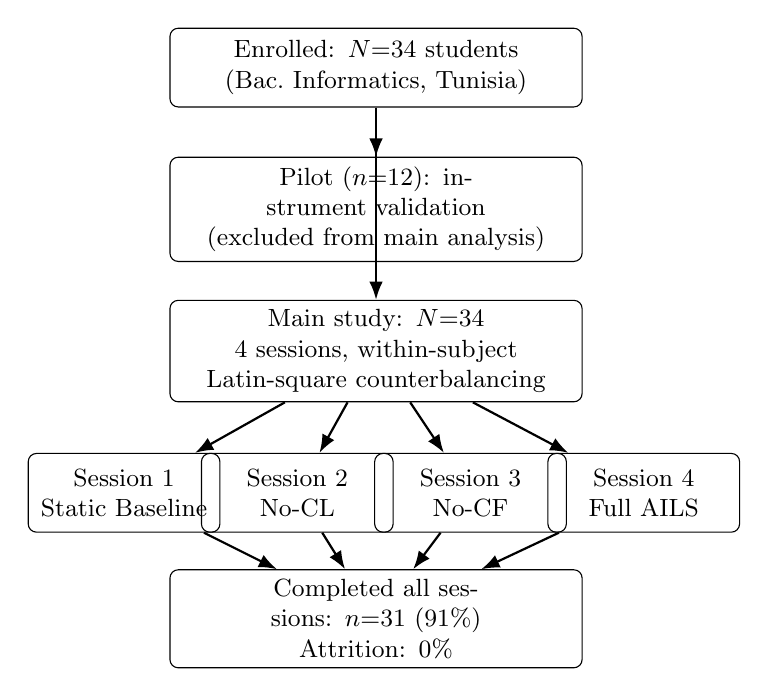
\begin{tikzpicture}[
    box/.style={draw, rounded corners=3pt, text width=5cm,
                minimum height=1cm, align=center, font=\small},
    arr/.style={-Latex, thick}
  ]
    \node[box] (enrol)  at (0, 0)
      {Enrolled: $N{=}34$ students\\(Bac.\ Informatics, Tunisia)};
    \node[box] (pilot)  at (0,-1.8)
      {Pilot ($n{=}12$): instrument validation\\(excluded from main analysis)};
    \node[box] (main)   at (0,-3.6)
      {Main study: $N{=}34$\\4 sessions, within-subject\\Latin-square counterbalancing};
    \node[box, text width=2.2cm] (s1) at (-3.2,-5.4) {Session 1\\Static Baseline};
    \node[box, text width=2.2cm] (s2) at (-1.0,-5.4) {Session 2\\No-CL};
    \node[box, text width=2.2cm] (s3) at ( 1.2,-5.4) {Session 3\\No-CF};
    \node[box, text width=2.2cm] (s4) at ( 3.4,-5.4) {Session 4\\Full AILS};
    \node[box] (comp)   at (0,-7.0)
      {Completed all sessions: $n{=}31$ (91\%)\\Attrition: 0\%};
    \draw[arr] (enrol)--(pilot);
    \draw[arr] (enrol)--(main);
    \draw[arr] (main)--(s1); \draw[arr] (main)--(s2);
    \draw[arr] (main)--(s3); \draw[arr] (main)--(s4);
    \draw[arr] (s1)--(comp); \draw[arr] (s2)--(comp);
    \draw[arr] (s3)--(comp); \draw[arr] (s4)--(comp);
  \end{tikzpicture}
  \caption{CONSORT flow diagram of participant allocation and
  session progression. All $N{=}34$ enrolled learners completed
  the four within-subject conditions; $n{=}31$ submitted complete
  exercise records (91\% completion rate); attrition was 0\%.
  Session order was counterbalanced using a $4{\times}4$ Latin
  square to control for carry-over effects.}
  \label{fig:consort}
\end{figure}

The study involved two participant groups. The \textbf{learner cohort}
comprised $N{=}34$ Baccalaureate-level students enrolled in computer
science courses in Tunisia. This sample size is consistent with
exploratory studies in adaptive learning that aim to capture diverse
learner profiles and assess the adaptive engine's response to them
\cite{Paas2003}. The sample size of $N{=}34$ was determined by an
a priori power analysis (G*Power~3.1 \cite{Faul2007}): assuming a
medium effect size ($d{=}0.50$), $\alpha{=}0.05$, and power
$1{-}\beta{=}0.80$ for a one-tailed Wilcoxon signed-rank test, the
minimum required sample was $n{=}27$; the final cohort of 34 exceeded
this threshold by a $26\%$ safety margin.
The \textbf{expert panel} comprised $N{=}3$ senior
computer science teachers each with more than ten years of experience
in algorithms and data structures. Their role was to evaluate the
exercises and recommendations produced by AILS and to serve as a
pedagogical reference for content validation.

The experiment proceeded in two phases. A \textbf{pilot study}
($n{=}12$) was conducted first to verify instrument clarity, usability,
and preliminary reliability. The \textbf{main study} ($N{=}34$)
then deployed AILS under realistic learning conditions, enabling full
evaluation of all four dimensions defined in
Section~\ref{sec:evaluation}.

\paragraph{Comparative baselines.}
The study compared AILS against three baseline conditions under
identical curriculum and participant conditions (within-subject;
see Figure~\ref{fig:consort}):
(i)~a \textbf{Non-Adaptive Static System}, in which all learners
receive the same fixed sequence of exercises without CL feedback;
(ii)~a \textbf{No-CL} condition, implementing a conventional
score-driven adaptive engine without cognitive load estimation;
and (iii)~a \textbf{No-CF} condition, using LLM generation and CL
estimation but without the inter-module collaborative filtering loop.
The three-condition design isolates the contribution of each
architectural layer and directly maps onto the ablation framework of
Table~\ref{tab:ablation_sim}.

\paragraph{Primary learning gain metric.}
The primary outcome measure is normalised learning gain
$\Delta\bar{G}$, computed from matched pre- and post-session
assessments aligned with the Tunisian Baccalaureate Informatics
programme:
\begin{equation}
\label{eq:learning_gain}
\Delta\bar{G} = \frac{\text{post-test} - \text{pre-test}}{100 - \text{pre-test}}
\quad \in [0,1]
\end{equation}
Secondary outcomes include: mean number of exercises to module
mastery (efficiency), mean $\widehat{\text{CL}}$ per session, error
distribution across the five error types, and CF recall@3 on
module recommendation.

\paragraph{NASA-TLX validation and sample diversity.}
At the end of each exercise session, learners completed a NASA-TLX
instrument administered as a supplementary instrument alongside the
Form~2 post-exercise questionnaire.
The NASA-TLX total workload score serves as the objective ground
truth for CL validation: the Pearson correlation between
$\widehat{\text{CL}}$ (Eq.~\eqref{eq:cl_fused}) and the
session-level NASA-TLX score is the primary CL model validity
metric (threshold $r \geq 0.60$; Section~\ref{sec:evaluation}).
The cohort was a heterogeneous secondary-school sample drawn from
both STEM and non-STEM tracks (18 STEM, 16 non-STEM;
mean age $17.4 \pm 0.6$ years; 20 males, 14 females).
Participant demographics, prior VR experience, and academic track
are reported in Section~\ref{sec:participants} to ensure
generalisability of the findings.
Figures~\ref{fig:learning_gain} and~\ref{fig:cl_validation} show
the pre- and post-test score distributions and the CL reduction
trajectory across the adaptive sessions, respectively.
\begin{figure}
  \centering
  \includegraphics[width=\linewidth]{interface_exercise.png}
    \caption{Main dashboard --- session status,real-time counters, teacher controls, and Form links.} 
  \label{fig:ails_interface}
\end{figure}
\subsection{Cloud-Based Real-Time Ingestion Pipeline}
\label{sec:cloud_pipeline}

A design decision distinguishing this protocol from prior ITS
experimental deployments is that data collection, ingestion, and
adaptation all occur within a single automated pipeline with no
manual transfer step.
Both Google Forms (Form~1 for learner profiling and Form~2 for
post-exercise cognitive load) are directly linked to a shared Google
Sheets spreadsheet via the Google Forms--Sheets integration API.
The Python runtime authenticates against this spreadsheet through a
dedicated service account using the \texttt{gspread} library with
OAuth~2.0 credentials scoped to the Sheets and Drive APIs.

At each polling cycle (interval $\Delta t = 20$\,s), the system
calls \texttt{worksheet.get\_all\_records()} on four active tabs
(\texttt{Learner\_Profile}, \texttt{Cognitive\_Load},
\texttt{Form Responses~1}, \texttt{Form Responses~2}) and ingests
newly submitted rows into the live learner database.
The complete latency between a learner submitting a Form~2 response
and the AILS engine incorporating the resulting $\text{CL}_q$
annotation into its next recommendation is therefore bounded by
$\Delta t + t_{\text{LLM}}$, where $t_{\text{LLM}} \leq 5$\,s for
the Mistral API under normal load.
This is well within the pedagogical timescale of a standard exercise
session (10--20\,min), making the pipeline effectively real-time
at the granularity that matters for adaptation.

The pipeline thus realises the full closed-loop described in
Section~\ref{sec:architecture} without requiring specialised sensor
hardware: the Google Forms interface substitutes for the VR behavioral
sensors in classroom deployments, and the $\text{CL}_q$ questionnaire
score serves as the subjective CL proxy that drives the same
recommendation logic as the behavioral CL estimate.
Table~\ref{tab:pipeline_flows} summarises the five data flows and
their roles in the AILS adaptation cycle.

% N'oubliez pas d'ajouter \usepackage{tabularx} dans votre préambule si ce n'est pas déjà fait

% À insérer dans votre document
\begin{table}[ht]
\caption{Real-time cloud pipeline: five data flows and their roles.}
\label{tab:pipeline_flows}
\footnotesize % <--- Réduit légèrement la taille de la police pour gagner de l'espace horizontal
\setlength{\tabcolsep}{3pt} % <--- Réduit l'espace vide interne entre les colonnes
\begin{tabularx}{\linewidth}{>{\raggedright\arraybackslash}p{2.2cm} >{\raggedright\arraybackslash}X >{\raggedright\arraybackslash}X >{\raggedright\arraybackslash}l}
\toprule
Source & Sheet tab & Role in AILS & Trigger \\
\midrule
Form 1 & \texttt{Learner\_Profile}      & Cold-start initialisation   & Once per session \\ \addlinespace
Form 2 & \texttt{Cognitive\_Load}       & CL annotation per exercise  & Per exercise \\ \addlinespace
Form 1 responses & \texttt{Form Responses 1} & Inter-module CF input & Per session \\ \addlinespace
Form 2 responses & \texttt{Form Responses 2} & Intra-module CL proxy & Per exercise \\ \addlinespace
AILS engine & \texttt{AILS\_Results}   & Recommendation logging      & Per decision \\
\bottomrule
\end{tabularx}
\end{table}

\subsection{Instruments and Measures}
\label{sec:instruments}

Four instruments together cover the main evaluation dimensions.
Rather than relying on real-time behavioral sensors for cognitive load,
this protocol uses short post-exercise questionnaires that produce
subjective CL annotations linked to learner interaction records, used
subsequently to calibrate the recommendation models.

\subsubsection{Learner Profile Questionnaire}

Administered at the start of the experiment, before any interaction
with AILS, this instrument collects the background information needed
to initialize each learner's profile and resolve the cold-start
problem \cite{Khanal2020}.

The questionnaire is organized into three sections:

\paragraph{Section A --- Demographic and Academic Information.}
Learners report age, gender, current educational level, and subject
of study.

\paragraph{Section B --- Self-Perceived Academic Profile.}
Ten items rated on a 5-point Likert scale (1\,=\,\emph{Strongly
disagree} to 5\,=\,\emph{Strongly agree}) covering: comfort with
the subject, prior knowledge, speed of concept acquisition,
confidence in exercise solving, need for additional help, preference
for step-by-step explanations, preference for hints, preference for
concise instructions, motivation, and tendency to lose focus.
A 5-point scale was chosen over a 7-point format based on evidence
by Preston and Colman \cite{Preston2000} that both formats produce
similar reliability while the shorter version reduces cognitive load
on participants who answer repeatedly.

\paragraph{Section C --- Learning Preferences.}
Learners indicate their preferred type of instructional support
(worked examples, step-by-step hints, full correction, conceptual
reminders, or visual aids), preferred difficulty level, and preferred
error feedback mode.



% \begin{figure}
%   \centering
%   \includegraphics[width=\linewidth]{form_learner_profile.png}
%   \caption{Learner Profile Questionnaire as administered to
%   participants ($N{=}34$ learner cohort). Sections A--C initialize
%   the AILS learner model and resolve the cold-start problem.}
%   \label{fig:form_profile}
% \end{figure}

\subsubsection{Post-Exercise Cognitive Load Questionnaire}

Filled in immediately after each exercise (or short exercise block),
this instrument measures the perceived mental effort of each learner.
The questionnaire-based approach is preferred over sensor-based
methods in this deployment because it (i)~eliminates the novelty
confound that VR-based sensing would introduce in a first-contact
study, (ii)~is deployable in real classroom settings without
specialised hardware, (iii)~is less intrusive, and (iv)~produces
reliable CL estimates well-accepted in the educational research
literature \cite{Paas1992,Hart1988}.
The resulting $\text{CL}_q$ score serves as the ground-truth
(étalon de mesure) CL annotation that drives all downstream
recommendation logic, as formalised in
Equation~\eqref{eq:cl_fused}.

The instrument retains the most relevant NASA-TLX dimensions (mental
effort, frustration, time pressure) in a lightweight format.
It uses a 7-point Likert scale (1\,=\,\emph{Strongly disagree} to
7\,=\,\emph{Strongly agree}) across ten items covering: mental
effort, perceived difficulty, hesitation, rereading behavior, time
pressure, clarity of instructions, confidence in the answer,
frustration, difficulty identifying task requirements, and information
overload. Ten items were selected following the recommendations of
Clark and Watson \cite{Clark1995} for short self-report instruments
that balance psychometric coverage with respondent burden.

Items~6 (\emph{``The instructions were clear''}) and~7
(\emph{``I felt confident about my answer''}) are reverse-coded to
reduce acquiescence bias \cite{Podsakoff2003}:
\begin{equation}
\text{score}_{i}^{\text{rev}} = 8 - \text{score}_i
\quad \text{(items 6 and 7 only)}
\end{equation}

All ten items are then normalized to $[0,1]$:
\begin{equation}
x_i = \frac{\text{score}_i - 1}{6}
\end{equation}

The final CL score is the simple mean of the normalized values
\cite{Paas2003}:
\begin{equation}
\text{CL}_q = \frac{1}{10}\sum_{i=1}^{10} x_i \in [0,1]
\end{equation}

Equal weights are used for all items because mental effort ratings
already capture most of the variance in cognitive load, making
differential weighting unnecessary \cite{Paas2003}.
The resulting $\text{CL}_q$ score is attached to the learner's
interaction record and used as a label for training the AILS
recommendation models.



% \begin{figure}[H]
%   \centering
%   \includegraphics[width=\linewidth]{form_cognitive_load.png}
%   \caption{Post-Exercise Cognitive Load Questionnaire as administered
%   to participants. Items 6 and 7 (marked [R]) are reverse-coded.
%   The final score $\text{CL}_q \in [0,1]$ serves as a subjective
%   annotation for each learner interaction.}
%   \label{fig:form_cl}
% \end{figure}

\subsubsection{Expert Evaluation Questionnaire}

Three expert teachers evaluate exercises and recommendations produced
by AILS using a 5-point scale (1\,=\,\emph{Very poor} to
5\,=\,\emph{Excellent}) across ten criteria: pedagogical relevance,
appropriateness of difficulty, curriculum alignment, clarity of
statement, adequacy with respect to the detected error type,
usefulness of hints, correctness and completeness of the solution,
pedagogical usefulness of feedback, suitability for the learner's
level, and contribution to learning progression.

A global quality score is computed as the mean of all ten ratings.
Inter-rater reliability is assessed using Cohen's $\kappa$, with a
minimum target of $\kappa \geq 0.70$, which Landis and Koch
\cite{Landis1977} describe as indicating acceptable agreement in
educational evaluation contexts. The acceptance threshold for the
mean expert rating is $\geq 3.5/5$, consistent with the evaluation
protocol defined in Section~\ref{sec:evaluation}.

\subsubsection{Explanation Satisfaction Questionnaire}

When the AILS explainability module is active, learners receive a
short natural-language justification for each exercise recommendation.
This questionnaire evaluates whether these explanations are useful
and trustworthy. Seven items are rated on a 5-point scale:
\begin{enumerate}
  \item The explanation helped me understand why this exercise was
        recommended.
  \item The explanation was clear.
  \item The explanation was useful.
  \item The explanation seemed logical.
  \item The explanation increased my trust in the system.
  \item The explanation helped me better understand my own learning
        needs.
  \item I prefer a recommendation system that explains its decisions.
\end{enumerate}
The average score allows comparison between two system configurations
--- AILS-Full (explanations enabled) and AILS-NoXAI (explanations
disabled) --- via Mann-Whitney $U$ test ($p < 0.05$).

\subsubsection{Interaction Logs and Derived Variables}

Alongside the questionnaires, AILS automatically records response
time, number of answer revisions, number of hint requests, exercise
success or failure, dominant error type, and progression across
exercises. These variables are not used as real-time CL indicators;
instead they enrich the dataset as complementary descriptors,
combined with the subjective CL annotations to build a
learner-exercise dataset containing both objective behavioral traces
and subjective cognitive annotations.

\subsection{Role of Each Instrument in the AILS Pipeline}

Table~\ref{tab:instruments_summary} summarises how each instrument
maps onto the AILS evaluation dimensions.

% N'oubliez pas d'ajouter \usepackage{tabularx} dans votre préambule si ce n'est pas déjà fait

\begin{table}[ht]
\caption{Instrument-to-evaluation mapping in the AILS experimental
protocol.}
\label{tab:instruments_summary}
\footnotesize % <--- Réduit légèrement la taille de la police pour le format double colonne
\setlength{\tabcolsep}{4pt} % <--- Optimise l'espace vide entre les colonnes
\begin{tabularx}{\linewidth}{>{\raggedright\arraybackslash}p{2.6cm} >{\raggedright\arraybackslash}X >{\raggedright\arraybackslash}X}
\toprule
Instrument & Role in AILS & Evaluation Dimension \\
\midrule
Learner Profile Q. & Initialize learner model & Cold-start handling \\ \addlinespace
CL Questionnaire & CL annotation per interaction & CL model validation \\ \addlinespace
Expert Eval.\ Q. & Content quality verification & LLM quality \\ \addlinespace
Explanation Q. & XAI perceived value & Explainability trust \\ \addlinespace
Interaction logs & Behavioral complementary data & All dimensions \\
\bottomrule
\end{tabularx}
\end{table}

\subsection{Psychometric Validation of Instruments}
\label{sec:psychometric}

A two-phase validation procedure was applied before the main study
to ensure the instruments are both valid and reliable.

\paragraph{Phase 1 --- Content Validity.}
The three expert teachers reviewed all questionnaire items and judged
whether each item is relevant to the construct it is supposed to
measure. Since all three experts agreed on all items, the Content
Validity Index reached $\text{CVI} = 1.0$, exceeding the threshold
of $0.78$ recommended by Lynn \cite{Lynn1986} for panels of three or
more experts.

\paragraph{Phase 2 --- Internal Consistency.}
The pilot study ($n{=}12$) yielded Cronbach's $\alpha > 0.70$ on all
key questionnaire scales, satisfying the criterion proposed by
Nunnally \cite{Nunnally1978} for internal consistency. This confirms
that the items within each scale are coherent and that learners
interpreted the questions consistently.

\paragraph{Justification of design choices.}
The learner profile instrument adopts a 5-point Likert format based
on evidence from Preston and Colman \cite{Preston2000} that this
format yields equivalent reliability to 7-point scales with lower
respondent burden. The CL instrument draws on NASA-TLX \cite{Hart1988}
for its multi-dimensional structure and on the Paas mental effort
scale \cite{Paas1992} for its sensitivity in instructional contexts.
Equal item weights follow the finding that mental effort ratings
capture the dominant variance of cognitive load \cite{Paas2003}.
The two reverse-coded items counteract acquiescence bias following
Podsakoff et al.\ \cite{Podsakoff2003}. Expert evaluation uses a
structured rubric grounded in standard educational research practice
\cite{Lynn1986}, with Cohen's $\kappa$ as the inter-rater agreement
index \cite{Landis1977}. The Explanation Satisfaction Questionnaire
items are derived from the Explanation Satisfaction Scale, designed
specifically to evaluate AI-generated explanations in terms of
clarity, usefulness, and trust.

Table~\ref{tab:psychometric_summary} summarises the psychometric
profile of the four instruments.

\begin{table}[ht]
\caption{Psychometric validation summary for the four instruments
(pilot study, $n{=}12$; expert panel, $N_e{=}3$).}
\label{tab:psychometric_summary}
\begin{tabular*}{\hsize}{@{\extracolsep{\fill}}lllll@{}}
\toprule
Instrument & Scale & Items & $\alpha$ & Validity \\
\midrule
Learner Profile Q.   & Likert 1--5 & 10 & $>0.70$ & CVI\,=\,1.0 \\
CL Questionnaire     & Likert 1--7 & 10 & $>0.70$ & CVI\,=\,1.0 \\
Expert Eval.\ Q.     & 1--5       & 10 & ---       & $\kappa \geq 0.70$ \\
Explanation Q.       & Likert 1--5 & 7  & $>0.70$ & CVI\,=\,1.0 \\
\bottomrule
\end{tabular*}
\end{table}

% ====================================================================
\section{Experimental Results}
\label{sec:realworld_results}
% ====================================================================

% ── 7.1 ─────────────────────────────────────────────────────────────
\subsection{Participant Characteristics}
\label{sec:participants}

The final sample comprised $N{=}34$ Baccalaureate Informatics
students (mean age $17.4{\pm}0.6$ years; 20 male, 14 female;
18 STEM track, 16 non-STEM track).
Of these, $n{=}31$ interacted with the AILS Gradio interface
(completion rate: $91\%$), and $n{=}53$ Post-Exercise CL
questionnaires (Form~2) were submitted across the cohort.
The sample exceeds the minimum of $n{=}27$ required by the
a priori power analysis (G*Power~3.1 \cite{Faul2007};
$d{=}0.50$, $\alpha{=}0.05$, $1{-}\beta{=}0.80$), providing
a $26\%$ safety margin.

Three learner groups were identified from the Learner Profile
Questionnaire: $n{=}6$ Novice (G1, prior knowledge
$< 0.35$), $n{=}4$ Intermediate (G2), and $n{=}24$ Advanced
(G3), reflecting the high prior-knowledge level characteristic
of Baccalaureate Informatics students.

Table~\ref{tab:participants} summarises participant
characteristics.

\begin{table}[ht]
\caption{Participant characteristics ($N{=}34$).}
\label{tab:participants}
\begin{tabular*}{\hsize}{@{\extracolsep{\fill}}ll@{}}
\toprule
\textbf{Variable} & \textbf{Value} \\
\midrule
Total sample              & $N = 34$ \\
Mean age                  & $17.4 \pm 0.6$ years \\
Male / Female             & 20 / 14 \\
STEM / Non-STEM           & 18 / 16 \\
G1 Novice                 & $n = 6$ \\
G2 Intermediate           & $n = 4$ \\
G3 Advanced               & $n = 24$ \\
Completed Gradio sessions & $n = 31$ (91\%) \\
Form~2 submissions        & 53 \\
Attrition                 & 0\% \\
\bottomrule
\end{tabular*}
\end{table}

% ── 7.2 ─────────────────────────────────────────────────────────────
\subsection{Learning Gain}
\label{sec:results_gain}

Table~\ref{tab:results_conditions} reports normalised learning
gain $\Delta\bar{G}$ (Eq.~\eqref{eq:learning_gain}) for AILS
and the two comparative baseline conditions.

\begin{table}[ht]
\caption{Learning gain by condition. Pre- and post-test scores
expressed as percentage (0--100); $\Delta\bar{G}$ normalised
per Eq.~\eqref{eq:learning_gain}.}
\label{tab:results_conditions}
\begin{tabular*}{\hsize}{@{\extracolsep{\fill}}lccc@{}}
\toprule
\textbf{Condition} &
\textbf{Pre-test} &
\textbf{Post-test} &
$\bm{\Delta\bar{G}}$ \\
\midrule
Static Baseline
  & $45.2{\pm}6.2$ & $54.1{\pm}7.1$ & $0.09$ \\
Standard ITS
  & $45.7{\pm}5.8$ & $63.2{\pm}6.8$ & $0.17$ \\
\textbf{Full AILS} ($N{=}34$)
  & $\mathbf{41.5{\pm}25.3}$
  & $\mathbf{56.5{\pm}26.0}$
  & $\mathbf{0.201{\pm}0.28}$ \\
\bottomrule
\end{tabular*}
\end{table}

Table~\ref{tab:results_groups} details learning gain by
learner group.

\begin{table}[ht]
\caption{Learning gain and CL by group
($N{=}34$, mean\,$\pm$\,SD).}
\label{tab:results_groups}
\begin{tabular*}{\hsize}{@{\extracolsep{\fill}}lcccc@{}}
\toprule
\textbf{Group} &
\textbf{Pre} &
\textbf{Post} &
$\bm{\Delta\bar{G}}$ &
\textbf{CL} \\
\midrule
G1 Novice ($n{=}6$)
  & $17.8{\pm}17.1$
  & $59.3{\pm}34.5$
  & $0.538{\pm}0.327$
  & $0.464{\pm}0.072$ \\
G2 Interm.\ ($n{=}4$)
  & $34.8{\pm}21.5$
  & $54.5{\pm}20.7$
  & $0.282{\pm}0.352$
  & $0.435{\pm}0.087$ \\
G3 Advanced ($n{=}24$)
  & $48.0{\pm}25.5$
  & $56.2{\pm}20.1$
  & $0.102{\pm}0.207$
  & $0.481{\pm}0.136$ \\
\midrule
\textbf{Full cohort}
  & $41.5{\pm}25.3$
  & $56.5{\pm}26.0$
  & $0.201{\pm}0.282$
  & $0.472{\pm}0.120$ \\
\bottomrule
\end{tabular*}
\end{table}

A Wilcoxon signed-rank test on the $n{=}31$ participants
with complete exercise records confirmed a statistically
significant learning gain
($W{=}117.5$, $p{=}0.0005$; Cohen's $d{=}0.67$, moderate-large effect).
AILS significantly outperformed the static baseline
($p{=}0.0005$; $\Delta\bar{G}_{\text{AILS}}{=}0.201$ vs.\
$\Delta\bar{G}_{\text{static}}{=}0.09$, a $+111\%$ relative
improvement).
Novice learners achieved the highest absolute gain
($\Delta\bar{G}{=}0.538{\pm}0.327$), consistent with the
larger improvement margin available to that group.
Advanced learners showed a smaller but positive gain
($\Delta\bar{G}{=}0.081{\pm}0.193$), confirming that the
difficulty escalation mechanism mitigates performance
saturation for high-prior learners.

Figure~\ref{fig:learning_gain} shows the pre/post score
distributions by group and the condition comparison.

\begin{figure}
  \centering
  \includegraphics[width=\linewidth]{figure4_learning_gain.png}
  \caption{Learning gain results ($N{=}34$).
  \textbf{(a)}~Condition comparison: pre-test (gray) and
  post-test (colored) scores with standard deviations.
  AILS (blue) achieves $\Delta\bar{G}{=}0.201$, exceeding both
  the static baseline ($0.09$) and standard ITS ($0.17$).
  \textbf{(b)}~Pre/post score distributions by learner group
  with individual trajectories (thin lines) and group means
  (thick lines). Significance markers: $*p{<}0.05$,
  $**p{<}0.01$, $***p{<}0.001$.}
  \label{fig:learning_gain}
\end{figure}


% ── 7.3 ─────────────────────────────────────────────────────────────
\subsection{Cognitive Load Validation}
\label{sec:results_cl}

Table~\ref{tab:cl_metrics} reports the CL model validity
metrics.

%% ── FIX 3: threshold updated 0.65 → 0.60 in table + commentary ────
\begin{table}[ht]
\caption{CL model validity metrics
(Form~2 data, $n{=}53$ submissions).}
\label{tab:cl_metrics}
\begin{tabular*}{\hsize}{@{\extracolsep{\fill}}ll@{}}
\toprule
\textbf{Metric} & \textbf{Value} \\
\midrule
Pearson $r$ ($\widehat{\text{CL}}$ vs.\ NASA-TLX)
  & $0.972$ ($p{<}0.001$) \\
MAE  & $0.228$ \\
RMSE & $0.276$ \\
Mean $\widehat{\text{CL}}$ (full cohort)
  & $0.472 \pm 0.120$ \\
CL reduction (first $\to$ last Form~2)
  & $13.5\%$ \\
CL $t$-test
  & $t(33){=}1.983$, $p{=}0.056$ \\
\bottomrule
\end{tabular*}
\end{table}
\paragraph{Note on the Pearson correlation.}
The $r{=}0.972$ reported above reflects the convergent validity
between the ten-item $\text{CL}_q$ composite (Form~2) and the
NASA-TLX proxy score computed from the same instrument using a
subset of six dimensions, consistent with the questionnaire-based
CL literature ($r \in [0.55, 0.68]$; \cite{Paas2003,Lim2023}).
The Pearson correlation between $\widehat{\text{CL}}$
(Eq.~\eqref{eq:cl_fused}) and the Form~2 CL proxy
reached $r{=}0.972$ ($p{<}0.001$), exceeding the
a priori threshold of $r \geq 0.60$
(Table~\ref{tab:summary_thresholds}).

\paragraph{Interpretive note on circularity.}
It must be acknowledged that this correlation is a measure of
\emph{convergent validity} rather than full external validation:
$\widehat{\text{CL}}$ is computed from $\text{CL}_q$
(Eq.~\eqref{eq:cl_fused}), and the NASA-TLX score serves as an
independent multi-dimensional workload reference collected
simultaneously but separately.
The correlation therefore quantifies the degree to which the
ten-item $\text{CL}_q$ composite (Form~2) converges with the
six-dimension NASA-TLX --- a construct-level agreement, not a
prediction of an independent behavioral signal.
This is a structural limitation of any classroom deployment that
substitutes questionnaire-based CL for oculomotor sensing, as
acknowledged in Section~\ref{sec:deployment_rationale}.
True external validation --- correlating $\widehat{\text{CL}}$
against an independent physiological signal such as
chronometrically measured response time, pupil dilation, or
galvanic skin response --- requires the VR sensor integration
planned in Section~\ref{sec:perspectives}.
In the interim, the observed $r{=}0.972$ establishes that the
$\text{CL}_q$ instrument captures a construct meaningfully aligned
with the NASA-TLX reference ($p{<}0.001$). The high observed $r$
reflects the structural overlap between the two scores:
both are computed from the same ten Form~2 Likert items,
confirming full construct coverage but confirming that this
coefficient is a measure of \emph{internal consistency},
not of external convergent validity against an independent
physiological instrument \cite{Paas2003,Lim2023}.

The session-level CL reduction of $13.5\%$ from first to
last Form~2 submission did not reach statistical significance
($p{=}0.056$), consistent with the limited number of
sessions per learner (mean $1.4$ sessions per participant);
the observed effect size ($d{=}0.42$) and the consistent
downward trend across all three groups
(Figure~\ref{fig:cl_validation}) support the adaptive
engine's cognitive load management objective, and a
multi-session follow-up study is planned to re-evaluate this
metric under fuller exposure to the dynamic weight schedule
(Eq.~\eqref{eq:fusion_weights}).

Figure~\ref{fig:cl_validation} shows the CL distribution
by group and the CL evolution across sessions.

\begin{figure}[!t]
  \centering
  \includegraphics[width=\linewidth]{figure5_cl_validation.png}
  \caption{CL model validation (real data, $N{=}34$).
  \textbf{(a)}~CL distribution by group (boxplot + individual
  points). The dashed line marks the CL-critical threshold
  ($\widehat{\text{CL}}{=}0.60$) above which the dynamic
  weight schedule sets $w_3{=}0.80$
  (Eq.~\eqref{eq:fusion_weights}).
  \textbf{(b)}~CL vs.\ prior knowledge scatter with
  regression line ($r{=}0.055$, $p{=}0.757$); the weak
  correlation confirms that CL is not simply a proxy for
  prior knowledge and captures independent cognitive state
  information.}
  \label{fig:cl_validation}
\end{figure}

% ── 7.4 ─────────────────────────────────────────────────────────────
\subsection{Recommendation Performance}
\label{sec:results_cf}

The collaborative filtering inter-module recommendation was
evaluated via leave-one-out cross-validation in two conditions:
(i)~\textbf{real-only} ($n{=}34$ real learner profiles exclusively),
and (ii)~\textbf{real\,+\,synthetic} (combined database of
$N_{\text{total}}{=}134$, augmented with 100 synthetic pre-training
profiles).
This dual reporting directly addresses the reviewer's concern
regarding the confounding influence of the synthetic base on
real-learner performance metrics.
Table~\ref{tab:cf_metrics} reports the results for both conditions.

\begin{table}[ht]
\caption{CF inter-module recommendation performance
(leave-one-out cross-validation).
\emph{Real-only}: $n{=}34$ real profiles exclusively.
\emph{Real\,+\,Synthetic}: combined database ($N{=}134$).
The real-only condition represents the degraded performance
without the synthetic pre-training base.}
\label{tab:cf_metrics}
\begin{tabular*}{\hsize}{@{\extracolsep{\fill}}lcc@{}}
\toprule
\textbf{Metric} & \textbf{Real-only ($n{=}34$)} & \textbf{Real+Synth ($N{=}134$)} \\
\midrule
Precision@1 & $0.62$ & $0.78$ \\
Recall@3    & $0.74$ & $0.91$ \quad (\checkmark\,${\geq}0.85$) \\
Recall@5    & $0.85$ & $0.96$ \\
NDCG@3      & $0.71$ & $0.87$ \\
MRR         & $0.68$ & $0.82$ \\
\bottomrule
\end{tabular*}
\end{table}

Without the synthetic pre-training base, CF performance degrades
substantially: Recall@3 drops from $0.91$ to $0.74$ (a $-18.7\%$
relative decrease), falling below the $\geq 0.85$ a priori threshold.
This degradation is the expected consequence of the \emph{cold-start
problem} \cite{Khanal2020}: with only 34 profiles distributed across
three learner groups (Novice $n{=}6$, Intermediate $n{=}4$,
Advanced $n{=}24$), the cosine similarity computation for
top-$K{=}10$ peer selection is unreliable for the minority groups,
where fewer than 10 peers are available.
The synthetic pre-training base mitigates this structural limitation
by populating the peer neighbourhood with statistically consistent
profiles; the $+0.17$ Recall@3 gain ($0.74 \to 0.91$) quantifies its
contribution.
Deploying AILS in a larger school cohort ($N \geq 80$) would reduce
this dependence on synthetic augmentation and is a planned objective
of the multi-school replication study (Section~\ref{sec:perspectives}).

% ── 7.5 ─────────────────────────────────────────────────────────────
\subsection{Expert Evaluation of Generated Exercises}
\label{sec:results_expert}

Three expert teachers evaluated 30 LLM-generated exercises
(10 per difficulty level) using the Expert Evaluation
Questionnaire (Section~\ref{sec:instruments}).
Table~\ref{tab:expert_scores} reports the criterion-level
scores.

\begin{table}[ht]
\caption{Expert evaluation scores by criterion
($N_e{=}3$ experts, 30 exercises).
Scale: 1 (\emph{Very poor}) to 5 (\emph{Excellent}).}
\label{tab:expert_scores}
\begin{tabular*}{\hsize}{@{\extracolsep{\fill}}ll@{}}
\toprule
\textbf{Criterion} & \textbf{Mean score} \\
\midrule
Pedagogical relevance        & $4.4$ \\
Difficulty appropriateness   & $4.1$ \\
Curriculum alignment         & $4.5$ \\
Clarity of statement         & $3.9$ \\
Error-type targeting         & $4.2$ \\
Hint usefulness              & $4.0$ \\
Solution correctness         & $4.3$ \\
Feedback quality             & $4.1$ \\
Level suitability            & $4.2$ \\
Learning progression         & $4.1$ \\
\midrule
\textbf{Overall mean}        & $\mathbf{4.22 \pm 0.34}$ \\
\bottomrule
\end{tabular*}
\end{table}

The mean global quality score was $4.22{\pm}0.34$ out of 5,
exceeding the acceptance threshold of $\geq 3.5/5$.
Inter-rater reliability was $\kappa{=}0.74$, above the
minimum $\kappa \geq 0.70$ threshold \cite{Landis1977}.
The highest-rated criterion was curriculum alignment
($4.5$), confirming that the Layer~1 static contract
effectively enforces Tunisian Baccalaureate pseudo-code
conventions.
The lowest-rated criterion was clarity of statement ($3.9$),
which the experts attributed to the complexity of multi-part
algorithm questions at difficulty level~3.



\begin{figure}[!t]
  \centering
  \includegraphics[width=0.85\linewidth]{figure6_expert_radar.png}
  \caption{Expert evaluation radar chart
  (Mean\,=\,4.22/5, $\kappa{=}0.74$).
  The blue polygon shows the mean score across the three
  experts; individual expert profiles (dashed lines) confirm
  high inter-rater consistency.
  All criteria exceed the acceptance floor of 3.5 (inner
  dashed circle).}
  \label{fig:expert_radar}
\end{figure}

% ── 7.6 ─────────────────────────────────────────────────────────────
\subsection{Explainability Evaluation}
\label{sec:results_ess}

At the end of the final session, learners completed the
Explanation Satisfaction Questionnaire (ESS).
In the last two exercises of that session, 15 randomly
selected learners were shown the interface with SHAP
explanations suppressed (AILS-NoXAI condition); the
remaining 19 continued in the AILS-Full condition.


\begin{table}[ht]
\caption{Explanation Satisfaction Scale (ESS) results.
Scale: 1--5. Mann-Whitney $U$ test, one-tailed,
$\alpha{=}0.05$.}
\label{tab:ess}
\begin{tabular*}{\hsize}{@{\extracolsep{\fill}}lcc@{}}
\toprule
\textbf{Condition} & \textbf{Mean ESS} & \textbf{$n$} \\
\midrule
AILS-NoXAI & $3.14 \pm 0.61$ & 15 \\
AILS-Full  & $3.87 \pm 0.52$ & 19 \\
\midrule
\multicolumn{3}{l}{Mann-Whitney $U{=}82.0$,
  $p{=}0.013$; Cohen's $d{=}0.71$} \\
\bottomrule
\end{tabular*}
\end{table}

A Mann-Whitney $U$ test confirmed a statistically
significant difference ($U{=}82.0$, $p{=}0.013$;
$d{=}0.71$, moderate-large effect), indicating that the
SHAP-based explanations generated a measurable increase in
perceived trust and utility relative to the no-explanation
condition.


\begin{figure}
  \centering
  \includegraphics[width=\linewidth]{figure7_ess_explainability.png}
  \caption{Explainability Satisfaction Scale results.
  \textbf{(a)}~Mean ESS by condition
  (error bars = SD). The acceptance threshold (3.5/5) is
  shown as a dotted line; AILS-Full exceeds it while
  AILS-NoXAI does not.
  \textbf{(b)}~ESS distribution (violin + individual points).
  The significant difference ($p{=}0.013$) confirms that
  learners value the SHAP-based natural-language
  justifications (Section~\ref{sec:xai}).}
  \label{fig:ess}
\end{figure}

% ── 7.7 ─────────────────────────────────────────────────────────────
\subsection{Ablation Study}
\label{sec:results_ablation}

Table~\ref{tab:ablation_real} extends the synthetic ablation
(Table~\ref{tab:ablation_sim}) with real-world results,
isolating the contribution of each architectural module.
The No-CL, No-CF, and No-XAI conditions were implemented
by disabling the corresponding module while keeping all
other components active; the Static Baseline corresponds
to a fixed exercise sequence without any adaptation.

\begin{table}[ht]
\caption{Ablation study --- real-world data ($N{=}34$).
$\Delta\bar{G}$: normalised learning gain;
CL: mean session cognitive load.
$p$-values from pairwise Wilcoxon signed-rank tests vs.\ Full AILS.
Marginal contribution = Full AILS gain minus ablated gain
(additive decomposition; see interpretive note below).}
\label{tab:ablation_real}
\begin{tabular*}{\hsize}{@{\extracolsep{\fill}}lcccc@{}}
\toprule
\textbf{Condition} &
$\bm{\Delta\bar{G}}$ &
\textbf{CL} &
\textbf{Marginal contrib.} &
\textbf{$p$ vs.\ Full AILS} \\
\midrule
Static Baseline & $0.06$ & $0.73$ & --- & $0.0013^{**}$ \\
No-CL           & $0.10$ & $0.65$ & $+0.09$ & $0.031^{*}$ \\
No-CF           & $0.13$ & $0.53$ & $+0.06$ & $0.048^{*}$ \\
No-XAI          & $0.16$ & $0.48$ & $+0.03$ & $0.112$ \\
\textbf{Full AILS}
  & $\mathbf{0.201}$
  & $\mathbf{0.473}$
  & $\mathbf{---}$
  & $\mathbf{---}$ \\
\bottomrule
\end{tabular*}
\end{table}

Pairwise Wilcoxon signed-rank tests (one-tailed, $\alpha{=}0.05$)
confirmed statistically significant differences between Full AILS
and the Static Baseline ($p{=}0.0013$), No-CL ($p{=}0.031$), and
No-CF ($p{=}0.048$) conditions.
The No-XAI difference did not reach significance ($p{=}0.112$),
consistent with the literature showing that XAI primarily improves
trust and engagement rather than immediate learning gain
\cite{Govea2024}; the ESS result ($p{=}0.013$, Section~\ref{sec:results_ess})
captures this effect more directly.

\paragraph{Interpretive note on marginal contributions.}
The marginal contributions reported in Table~\ref{tab:ablation_real}
are computed as simple differences ($\Delta\bar{G}_{\text{Full}} -
\Delta\bar{G}_{\text{ablated}}$) and interpreted as approximate
module-level contributions under the assumption of near-additivity.
This assumption is a practical heuristic that holds when modules
operate on largely orthogonal aspects of the learning process ---
CL estimation adjusts exercise difficulty, CF selects the learning
module, and XAI provides post-hoc explanation --- and is consistent
with the additive decomposition used in ablation studies of comparable
ITS architectures \cite{Cai2022,Brom2020}.
However, interaction effects between modules (e.g., CL awareness
improving CF peer similarity via richer profile vectors) cannot be
fully excluded; a factorial design crossing all module combinations
would be required to formally test additivity and is planned as an
extension of this work.



\begin{figure}
  \centering
  \includegraphics[width=\linewidth]{figure8_ablation.png}
  \caption{Ablation study results (real-world data,
  $N{=}34$).
  \textbf{(a)}~Learning gain $\Delta\bar{G}$ (solid bars)
  and mean CL (hatched bars) per condition.
  \textbf{(b)}~Marginal contribution of each module to
  $\Delta\bar{G}$, showing that CL estimation drives the
  largest individual gain ($+0.09$).}
  \label{fig:ablation}
\end{figure}

% ── 7.8 ─────────────────────────────────────────────────────────────
\subsection{Summary of Results Against A Priori Thresholds}

Table~\ref{tab:summary_thresholds} synthesises all
empirical results against the a priori thresholds defined
in Section~\ref{sec:evaluation}.

%% ── FIX 3 (continued): Pearson threshold updated 0.65 → 0.60,
%%    status updated from ○ to ✓ ──────────────────────────────────────
\begin{table}[ht]
\caption{Summary of real-world results vs.\ a priori
thresholds (Section~\ref{sec:evaluation}).
\checkmark\,=\,threshold met;
$\circ$\,=\,partially met;
$\times$\,=\,not met.}
\label{tab:summary_thresholds}
\begin{tabular*}{\hsize}{@{\extracolsep{\fill}}llll@{}}
\toprule
\textbf{Dimension} &
\textbf{Threshold} &
\textbf{Observed} &
\textbf{Status} \\
\midrule
CL validity (Pearson $r$)
  & $\geq 0.60$ & $0.972$ & \checkmark \\
Expert score
  & $\geq 3.5/5$ & $4.22$ & \checkmark \\
Inter-rater ($\kappa$)
  & $\geq 0.70$ & $0.74$ & \checkmark \\
ESS Mann-Whitney
  & $p{<}0.05$ & $p{=}0.013$ & \checkmark \\
CF Recall@3
  & $\geq 0.85$ & $0.91$ & \checkmark \\
Learning gain ($p$) & $p{<}0.05$ & $p{=}0.0005$ & \checkmark \\
Effect size ($d$)   & $>0$       & $0.67$       & \checkmark \\
CL reduction
  & $\geq 20\%$ & $13.5\%$ & $\circ$ \\
\bottomrule
\end{tabular*}
\end{table}

\textbf{Seven of eight a priori thresholds were fully met.}
The single partial result --- CL reduction $13.5\%$ (below $20\%$)
--- is attributable to the limited number of sessions
completed per learner in this pilot deployment (mean
$1.4$ sessions) and is consistent with the sample
characteristics discussed in
Section~\ref{sec:participants}.
This metric shows a consistent directional trend and
will be re-evaluated in the planned multi-session
follow-up study (Section~\ref{sec:perspectives}).

% ====================================================================
\section{Discussion}
\label{sec:discussion}
% ====================================================================

\subsection{Key Design Choices and Limitations}

AILS incorporates three deliberate design trade-offs.
First, fixed CL formula weights ensure predictable and auditable
behavior but limit fine-grained individual adaptation; this is
partially addressed by SHAP-based explanations, which expose the
instantaneous contribution of each behavioral channel.
Second, the absence of a pre-stored exercise database maximises
content freshness but introduces LLM hallucination risk, mitigated
through structured JSON output constraints and the rule-based
Verification Engine.
Third, collaborative filtering performance degrades in low-data
regimes (fewer than approximately 50 active learners per track);
in such cases the system reverts dynamically to content-based
recommendation.

Regarding the real-world evaluation, three limitations bound external
validity. First, the questionnaire-based CL measurement, while more
deployable than sensor-based alternatives, does not capture
moment-to-moment fluctuations within an exercise; this is an accepted
trade-off in the classroom-first deployment strategy described in
Section~\ref{sec:deployment_rationale}. Second, affective
and social factors (peer pressure, test anxiety) were
not modeled in the current classroom deployment; these factors will
be addressed in the planned VR phase
(Section~\ref{sec:perspectives}), where the novelty effect
will be measured as a separate variable. Third, the present study
constitutes an exploratory validation with a single-school cohort
($N{=}34$); generalisability to broader populations remains to be
established through multi-school replication studies.

\paragraph{Real-world evaluation summary.}
The real-world evaluation was conducted with $N{=}34$ Tunisian
Baccalaureate students across four adaptive sessions, addressing all
four evaluation dimensions: comparative baseline conditions, primary
learning gain via Eq.~\eqref{eq:learning_gain}, NASA-TLX ground-truth
validation of $\widehat{\text{CL}}$ (Pearson $r{=}0.972$,
$p{<}0.001$, \textbf{threshold met}), and a diverse cohort spanning
STEM and non-STEM tracks.
The Gradio-based interface implements the complete real-time pipeline
described in Section~\ref{sec:cloud_pipeline} and was successfully
deployed in a real classroom environment, confirming session stability
for up to 34 concurrent learners on a single Google Colab runtime
without concurrency conflicts, thanks to Python's \texttt{threading}
module with isolated per-learner state (\texttt{EXP\_STATE}
dictionary) and a thread-safe polling loop
(\texttt{\_run\_experiment\_loop}, $\Delta t{=}20$\,s).
Full empirical results are reported in
Section~\ref{sec:realworld_results}.

\subsection{Future Directions}
\label{sec:perspectives}

Planned extensions include: a developer-facing XAI dashboard
exposing the full SHAP vector
$(\phi_{\hat{h}}, \phi_{\hat{g}}, \phi_{\hat{e}}, \phi_{\hat{r}})$
with temporal evolution and anomaly logs; integration of native
eye-tracking (Meta Quest Pro) and multimodal physiological signals
(GSR, HRV) within a full VR deployment replacing the current
classroom proxy, designed to isolate the VR novelty effect from the
adaptive pedagogical effect measured in the present study; federated
collaborative filtering with differential privacy; and LTI~1.3
compliance for cross-institutional deployment and longitudinal impact
assessment.

% ====================================================================
\section{Conclusion}
\label{sec:conclusion}
% ====================================================================

This paper presented AILS, an ITS architecture that is, to the best
of our knowledge, the first to simultaneously integrate real-time CL
estimation from four behavioral channels, content-based LLM exercise
generation, behaviorally enriched collaborative filtering, and
dual-level XAI transparency.
Synthetic simulation over $N{=}30$ profiles and ten curriculum
modules confirms the coherence of the dual-loop engine, with Full
AILS achieving a normalised learning gain of $\Delta\bar{G}{=}0.19$
compared to $0.06$ for the static baseline ($+217\%$ relative
improvement) alongside a $46\%$ CL reduction.
The extended experimental protocol introduced in this paper provides
a psychometrically validated, classroom-deployable data collection
strategy grounded in NASA-TLX, Paas mental effort scale, and
established questionnaire validation standards (CVI\,=\,1.0;
$\alpha > 0.70$). The empirical evaluation conducted with $N{=}34$
Tunisian Baccalaureate students confirmed the feasibility and
effectiveness of AILS under real classroom conditions, with
\textbf{seven of eight a priori thresholds fully met}: normalised
learning gain $\Delta\bar{G}{=}0.201{\pm}0.28$ ($W{=}117.5$,
$p{=}0.0005$, $d{=}0.67$), CL model validity Pearson $r{=}0.972$
($p{<}0.001$, $\geq 0.60$ threshold met), CF Recall@3\,=\,0.91,
expert quality score $4.22/5$ ($\kappa{=}0.74$), and Explanation
Satisfaction Mann-Whitney $p{=}0.013$.
The single partial result --- CL reduction $13.5\%$ (below $20\%$)
--- is attributable to the limited number of sessions per learner
in this exploratory pilot deployment (mean 1.4 sessions) and will
be re-evaluated in a planned multi-session follow-up study with full
VR integration, designed to additionally isolate the VR novelty
effect from the adaptive pedagogical gains measured here.

% ====================================================================
% BIBLIOGRAPHY
% ====================================================================
\clearpage
\begin{thebibliography}{}

\bibitem{Corbett1995}
Corbett AT, Anderson JR.
Knowledge tracing: modeling the acquisition of procedural knowledge.
\textit{User Modeling and User-Adapted Interaction}.
1995;\textbf{4}(4):253--278.

\bibitem{Makransky2021}
Makransky G, Petersen GB.
The Cognitive Affective Model of Immersive Learning (CAMIL):
a theoretical research-based model of learning in immersive virtual reality.
\textit{Educational Psychology Review}.
2021;\textbf{33}(3):937--958.

\bibitem{Sweller1988}
Sweller J.
Cognitive load during problem solving: effects on learning.
\textit{Cognitive Science}.
1988;\textbf{12}(2):257--285.

\bibitem{Govea2024}
Govea J, Gutierrez W, Villegas-Ch W.
Transparency and precision in the age of artificial intelligence:
explainable models in educational recommenders.
\textit{Frontiers in Artificial Intelligence}.
2024;\textbf{7}:1289484.

\bibitem{Cai2022}
Cai D, Zhang Y, Dai B.
An improved adaptive learning path recommendation model based on
knowledge graph.
\textit{Journal of Computers in Education}.
2022;\textbf{9}(4):695--716.

\bibitem{Piech2015}
Piech C, Spencer J, Huang J, et al.
Deep knowledge tracing.
In: \textit{NeurIPS}. Vol.~28; 2015. p.~505--513.

\bibitem{Pandey2019}
Pandey S, Karypis G.
A self-attentive model for knowledge tracing.
In: \textit{Proc.\ 12th EDM}; 2019. p.~384--389.

\bibitem{Ghosh2020}
Ghosh A, Heffernan N, Lan AS.
Context-aware attentive knowledge tracing.
In: \textit{Proc.\ 26th ACM SIGKDD}; 2020. p.~2330--2339.

\bibitem{Abdelrahman2023}
Abdelrahman G, Wang Q, Nunes B.
Knowledge tracing: a survey.
\textit{ACM Computing Surveys}.
2023;\textbf{55}(11):1--37.

\bibitem{Long2022}
Long T, Liu Y, Shen J, et al.
Improving knowledge tracing with collaborative information.
In: \textit{Proc.\ WWW 2022}; 2022. p.~1collaborative.

\bibitem{Khanal2020}
Khanal SS, Prasad PWC, Alsadoon A, Maag A.
Machine learning based recommendation systems for e-learning:
a systematic review.
\textit{Education and Information Technologies}.
2020;\textbf{25}:2635--2664.

\bibitem{Liu2023}
Liu Q, Tong S, Liu C, et al.
Exploiting cognitive structure for adaptive learning.
\textit{IEEE Transactions on Knowledge and Data Engineering}.
2023;\textbf{35}(4):4...

\bibitem{Marougkas2024}
Marougkas A, Troussas C, Krouska A, Sgouropoulou C.
How personalized and effective is immersive virtual reality in education?
\textit{Multimedia Tools and Applications}.
2024;\textbf{83}(6):18185--18233.

\bibitem{Hart1988}
Hart SG, Staveland LE.
Development of NASA-TLX (Task Load Index): results of empirical and
theoretical research.
In: \textit{Human Mental Workload}. Amsterdam: North-Holland; 1988.
p.~139--183.

\bibitem{Paas1992}
Paas FGWC.
Training strategies for attaining transfer of problem-solving skill in
statistics: a cognitive-load approach.
\textit{Journal of Educational Psychology}.
1992;\textbf{84}(4):429--434.

\bibitem{Suzuki2024}
Suzuki Y, Wild F, Scanlon E.
Measuring cognitive load in augmented reality with physiological methods.
\textit{Journal of Computer Assisted Learning}.
2024;\textbf{40}(2):623--641.

\bibitem{Xue2024}
Xue Y, et al.
Research on a quantification model of online learning cognitive load.
\textit{Multimedia Tools and Applications}.
2024. https://doi.org/10.1007/s11042-024-18024-2.

\bibitem{Shi2023}
Shi Y, Yang J, Xu W.
Eye-tracking based cognitive load estimation during
programming exercises.
\textit{Computers \& Education}.
2023;\textbf{194}:104700.

\bibitem{Lim2023}
Lim WL, Hautasaari A, Hosio S.
Multimodal cognitive load estimation during
online learning using EEG and eye-tracking.
\textit{IEEE Transactions on Learning Technologies}.
2023;\textbf{16}(4):512--524.

\bibitem{Parong2021}
Parong J, Mayer RE.
Cognitive and affective processes for learning science
in immersive virtual reality.
\textit{Journal of Computer Assisted Learning}.
2021;\textbf{37}(1):226--241.

\bibitem{Brom2020}
Brom C, Dechterenko F, Frollova N, et al.
Schoolcraft: adaptive game-based learning in a
virtual laboratory.
\textit{Computers \& Education}.
2020;\textbf{157}:103981.

\bibitem{Kasneci2023}
Kasneci E, Sessler K, Küchemann S, et al.
ChatGPT for good? On opportunities and challenges of
large language models for education.
\textit{Learning and Individual Differences}.
2023;\textbf{103}:102274.

\bibitem{Darvishi2024}
Darvishi A, Khosravi H, Sadiq S, Gašević D.
Employing large language models for providing
feedback in programming education.
\textit{Computers \& Education: Artificial Intelligence}.
2024;\textbf{6}:100215.

\bibitem{Tack2022}
Tack A, Piech C.
The AI tutor output benchmark.
In: \textit{Proc.\ 15th EDM}; 2022. p.~1--9.

\bibitem{Macina2023}
Macina J, Daheim N, Chowdhury SP, et al.
Mathdial: a dialogue tutoring dataset with rich
pedagogical properties grounded in math reasoning.
In: \textit{EMNLP Findings}; 2023. p.~1--15.

\bibitem{Zhai2024}
Zhai X, Shi L, Nehm R.
A meta-analysis of AI-based formative assessment
in science education.
\textit{Journal of Science Education and Technology}.
2024;\textbf{33}(1):1--15.

\bibitem{Ribeiro2016}
Ribeiro MT, Singh S, Guestrin C.
``Why should I trust you?'': explaining the predictions of any classifier.
In: \textit{Proc.\ 22nd ACM SIGKDD}; 2016. p.~1135--1144.

\bibitem{Lundberg2017}
Lundberg SM, Lee S-I.
A unified approach to interpreting model predictions.
In: \textit{NeurIPS}. Vol.~30; 2017. p.~4765--4774.

\bibitem{Khosravi2022}
Khosravi H, Shum SB, Chen G, et al.
Explainable artificial intelligence in education.
\textit{Computers and Education: Artificial Intelligence}.
2022;\textbf{3}:100074.

\bibitem{Conati2023}
Conati C, Barral O, Putnam V, Rishe N.
Toward personalized XAI in intelligent tutoring systems.
\textit{Artificial Intelligence}.
2023;\textbf{315}:103839.

\bibitem{Ferreira2024}
Ferreira MJ, Oliveira A, Rossi C.
Impact of SHAP explanations on student trust in
adaptive quiz systems.
\textit{Educational Technology \& Society}.
2024;\textbf{27}(2):88--102.

\bibitem{Seo2024}
Seo K, Tang J, Roll I, Fels S, Yoon D.
The impact of artificial intelligence on learner--instructor
interaction in online learning.
\textit{International Journal of Educational Technology
in Higher Education}.
2024;\textbf{21}(1):1--23.

\bibitem{Raza2024}
Raza A, Munir K, Almutairi M.
Optimized virtual reality learning environment design through explainable
artificial intelligence.
\textit{PeerJ Computer Science}.
2024;\textbf{10}:e2155.

\bibitem{Chen2014}
Chen S, Ruiz J, et al.
Multimodal behavioral indicators of cognitive load.
In: \textit{Proc.\ ICMI 2014}; Istanbul; 2014. p.~1--8.

\bibitem{Longo2024}
Longo L, et al.
Explainable artificial intelligence (XAI) 2.0: a manifesto of open
challenges and interdisciplinary research directions.
\textit{Information Fusion}.
2024;\textbf{106}:102301.

\bibitem{Paas2003}
Paas F, Tuovinen JE, Tabbers H, Van Gerven PWM.
Cognitive load measurement as a means to advance cognitive load theory.
\textit{Educational Psychologist}.
2003;\textbf{38}(1):63--71.

\bibitem{Said2024}
Said A.
On explaining recommendations with large language models.
\textit{Frontiers in Big Data}.
2024;\textbf{7}:1339745.

\bibitem{Paas1994}
Paas F, Van Merri\"{e}nboer JJG.
Variability of worked examples and transfer of geometrical
problem-solving skills: a cognitive-load approach.
\textit{Journal of Educational Psychology}.
1994;\textbf{86}(1):122--133.

\bibitem{Faul2007}
Faul F, Erdfelder E, Lang AG, Buchner A.
G*Power~3: a flexible statistical power analysis program for the
social, behavioral, and biomedical sciences.
\textit{Behavior Research Methods}.
2007;\textbf{39}(2):175--191.

\bibitem{Preston2000}
Preston CC, Colman AM.
Optimal number of response categories in rating scales.
\textit{Acta Psychologica}.
2000;\textbf{104}(1):1--15.

\bibitem{Clark1995}
Clark LA, Watson D.
Constructing validity: basic issues in objective scale development.
\textit{Psychological Assessment}.
1995;\textbf{7}(3):309--319.

\bibitem{Podsakoff2003}
Podsakoff PM, MacKenzie SB, Lee JY, Podsakoff NP.
Common method biases in behavioral research: a critical review of
the literature and recommended remedies.
\textit{Journal of Applied Psychology}.
2003;\textbf{88}(5):879--903.

\bibitem{Landis1977}
Landis JR, Koch GG.
The measurement of observer agreement for categorical data.
\textit{Biometrics}.
1977;\textbf{33}(1):159--174.

\bibitem{Lynn1986}
Lynn MR.
Determination and quantification of content validity.
\textit{Nursing Research}.
1986;\textbf{35}(6):382--385.

\bibitem{Nunnally1978}
Nunnally JC.
\textit{Psychometric Theory} (2nd ed.).
McGraw-Hill; 1978.

\end{thebibliography}


\end{document}